%%%%%%%%%%%%%%%%%%%%%%%%%%%%%%%%%%%%%%%%%%%%%%%%%%%
%% Modèle de rapport pédagogique, doublé d'un tutoriel LaTeX
%% Vincent Labatut 2014-20 <vincent.labatut@univ-avignon.fr>
%%%%%%%%%%%%%%%%%%%%%%%%%%%%%%%%%%%%%%%%%%%%%%%%%%%
%% Classe du document
\documentclass{ceri/sty/rapport}
% \documentclass[handout]{ceri/sty/rapport}
% \documentclass[light]{ceri/sty/rapport}
% \documentclass[full]{ceri/sty/rapport}
% \documentclass[blue]{ceri/sty/rapport}





%%%%%%%%%%%%%%%%%%%%%%%%%%%%%%%%%%%%%%%%%%%%%%%%%%%
%% Paquetes adicionales necesarios
%%%%%%%%%%%%%%%%%%%%%%%%%%%%%%%%%%%%%%%%%%%%%%%%%%%
\usepackage{booktabs}       % \toprule, \midrule, \bottomrule (tablas de publicación)
\usepackage{longtable}      % tablas que pueden ocupar varias páginas
\usepackage{threeparttable} % notas al pie de tabla integradas (opcional, para \fuente / \nota)
\usepackage{siunitx}
\sisetup{
	output-decimal-marker = {,},
	group-separator = {.},
	group-minimum-digits = 4,
	group-digits = integer,
}
\usepackage{mathtools}
\usepackage[spanish,nameinlink,noabbrev]{cleveref}
%% NOTA: NO cargar natbib, titlesec, caption, subcaption, hyperref, etc.: rapport.cls ya los carga.

%% Correcciones de cabecera (el título largo excede 14pt)
\setlength{\headheight}{28pt}

%% La fuente Gilroy no tiene versalitas: evitar warnings/errores
\renewcommand{\textsc}[1]{\textnormal{#1}}
\renewcommand{\textsl}[1]{\textit{#1}}

%% Silenciar warning de todonotes (lo carga la clase con margen estrecho)
\setlength{\marginparwidth}{2cm}

%% Permitir saltos de línea limpios en nombres de archivo/ruta largos
\makeatletter
\g@addto@macro\UrlBreaks{\do\_\do\-}
\makeatother
\newcommand{\archivo}[1]{\nolinkurl{#1}}





%%%%%%%%%%%%%%%%%%%%%%%%%%%%%%%%%%%%%%%%%%%%%%%%%%%
%% Informations générales
%%%%%%%%%%%%%%%%%%%%%%%%%%%%%%%%%%%%%%%%%%%%%%%%%%%
%TODO Formation concernée : à compléter.
\major{Ciclo}

%TODO Parcours ou spécialité de la formation
\specialization{VIII}

%TODO UE concernée par le rapport (à modifier).
\course{Procesos Estocásticos}

%TODO UCE concernée par le rapport (à modifier, optionnel).
\subcourse{FACULTAD DE NEGOCIOS}

%TODO Titre du document, à adapter.
\title{Predicción de las revisiones del PBI peruano mediante modelos econométricos, aprendizaje automático y computación de reservorio cuántico}
\makeatletter
\def\subtitle#1{\gdef\MySubtitle{#1}}
\makeatother
\subtitle{Evaluación empírica, simulación calibrada y análisis en tiempo real, 1994--2025}

%TODO Liste des auteurs
\author{
	Arriaga Velasquez Stephany \\
	Bellido León Angel \\
	Quispe Rodriguez Cleison \\
	Velasquez Ruiz Leonardo \\
	Vilchez Laiza Mariano
}

%TODO Liste des encadrants, responsables d'UE, etc. (optionnel)
\advisor[Docente]{
	Ventura Aguilar, Henry 
}

%TODO Groupe des auteurs
\group{Grupo D}

%\date{\today}

\summary{Cuando se publica por primera vez el crecimiento mensual del Producto Bruto Interno (PBI) del Perú, la cifra es preliminar y suele corregirse en los meses siguientes conforme llegan nuevas encuestas y registros. Este trabajo evaluó si un modelo de computación de reservorio cuántico (QRC) logra anticipar esas correcciones futuras mejor que los modelos estadísticos y de aprendizaje automático tradicionales, usando únicamente la información disponible en cada mes. Para comprobarlo, se revisaron \(44\,307\) registros históricos entre 1994 y 2025, se construyó una serie limpia sin saltos metodológicos a un horizonte fijo de once meses (\(n=350\)) y se evaluaron doce modelos sobre \(250\) pronósticos mensuales entre 2003 y 2024, reservando los últimos sesenta meses como prueba final. Los resultados muestran que las primeras cifras del PBI subestiman sistemáticamente el dato corregido en \(+0{,}35\) puntos porcentuales en promedio y presentan un patrón anual reconocible. Sin embargo, el modelo cuántico (\(\text{RMSE}=0{,}478\)) no superó a sus equivalentes clásicos no lineales: empató estadísticamente con una red clásica de reservorio (\(\text{RMSE}=0{,}472\)) y quedó por debajo de las características aleatorias de Fourier (\(\text{RMSE}=0{,}456\)) y de los árboles de decisión durante la pandemia (\(\text{RMSE}=0{,}349\) frente a \(0{,}363\)). En doce escenarios simulados tampoco apareció ninguna condición donde el enfoque cuántico ganara con claridad. Siguiendo la regla establecida antes de iniciar las pruebas, no se atribuyó superioridad al modelo cuántico ni se realizó la valoración económica condicionada.\\
\textbf{Palabras clave:} revisiones del PBI; datos en tiempo real; computación de reservorio cuántico; pronóstico económico; aprendizaje automático.}






%%%%%%%%%%%%%%%%%%%%%%%%%%%%%%%%%%%%%%%%%%%%%%%%%%%
%% Bibliografía
%%%%%%%%%%%%%%%%%%%%%%%%%%%%%%%%%%%%%%%%%%%%%%%%%%%
%% La clase ya carga biblatex con backend=biber.
%% El archivo debe llamarse exactamente como aquí abajo.
%% Compilar con: lualatex → biber → lualatex → lualatex
\addbibresource{bibliographie.bib}





%%%%%%%%%%%%%%%%%%%%%%%%%%%%%%%%%%%%%%%%%%%%%%%%%%%
%% Colores de los cuatro países (iguales en tablas y gráficos)
%%%%%%%%%%%%%%%%%%%%%%%%%%%%%%%%%%%%%%%%%%%%%%%%%%%
\definecolor{cDEU}{HTML}{1F4E79}
\definecolor{cBRA}{HTML}{2E8B57}
\definecolor{cIND}{HTML}{E07B00}
\definecolor{cHTI}{HTML}{B22222}
\definecolor{cGRIS}{HTML}{A6A6A6}
\definecolor{cSOC}{HTML}{2F6DB5}
\definecolor{cINT}{HTML}{C0392B}
\definecolor{cDEF}{HTML}{6B6B66}
\definecolor{cSAL}{HTML}{8E44AD}
\definecolor{cCAP}{HTML}{27AE60}





%%%%%%%%%%%%%%%%%%%%%%%%%%%%%%%%%%%%%%%%%%%%%%%%%%%
%% Utilidades
%%%%%%%%%%%%%%%%%%%%%%%%%%%%%%%%%%%%%%%%%%%%%%%%%%%
\newcommand{\fuente}[1]{\par\vspace{3pt}{\footnotesize\raggedright Fuente: #1\par}}
\newcommand{\nota}[1]{\par\vspace{1pt}{\footnotesize\raggedright #1\par}}
\newcommand{\bloque}[2]{\multicolumn{#1}{@{}l}{\textit{#2}}\\}

\newcommand{\recuadro}[2]{\par\medskip\noindent
	\fcolorbox{cDEU}{cDEU!5}{%
		\begin{minipage}{\dimexpr\linewidth-2\fboxsep-2\fboxrule\relax}
			\linespread{1.2}\selectfont\small\textbf{#1}\par\smallskip #2%
	\end{minipage}}%
	\par\medskip}

\setlength{\parskip}{0.2em}

\renewcommand{\topfraction}{0.85}
\renewcommand{\bottomfraction}{0.6}
\renewcommand{\textfraction}{0.1}
\renewcommand{\floatpagefraction}{0.7}
\setcounter{topnumber}{3}
\setcounter{totalnumber}{4}
\makeatletter
\setlength{\@fptop}{0pt}
\setlength{\@fpsep}{18pt plus 4pt}
\setlength{\@fpbot}{0pt plus 1fil}
\makeatother

%% Definiciones matemáticas para el contenido de Inves.tex
\newcommand{\PBI}{\text{PBI}}
\newcommand{\RMSE}{\text{RMSE}}
\newcommand{\MAE}{\text{MAE}}
\newcommand{\DM}{\text{DM}}
\newcommand{\QRC}{\text{QRC}}
\newcommand{\ESN}{\text{ESN}}
\newcommand{\DFM}{\text{DFM}}
\newcommand{\E}{\mathbb{E}}
\newcommand{\R}{\mathbb{R}}

%% IMPORTANTE: rapport.cls ya define \newtheorem{definition}{Definition}.
%% No volver a definirla. Solo definimos los teoremas que NO existen en la clase.
\theoremstyle{definition}
\newtheorem{assumption}{Supuesto}
\newtheorem{hypothesis}{Hipótesis}





%%%%%%%%%%%%%%%%%%%%%%%%%%%%%%%%%%%%%%%%%%%%%%%%%%%
%% Début du document
%%%%%%%%%%%%%%%%%%%%%%%%%%%%%%%%%%%%%%%%%%%%%%%%%%%
\begin{document}
	
	\maketitle
	
	\sloppy
	
	%%%%%%%%%%%%%%%%%%%%%%%%%%%%%%%%%%%%%%%%%%%%%%%%%%%
	%% SECCIONES MODULARES
	%%%%%%%%%%%%%%%%%%%%%%%%%%%%%%%%%%%%%%%%%%%%%%%%%%%
	% ============================================================================
\section{Introducción y marco metodológico}

Seguir de cerca la economía es fundamental para tomar decisiones públicas y empresariales, pero los responsables deben actuar casi siempre con cifras preliminares. En el caso del Producto Bruto Interno (PBI) mensual, la primera cifra que se publica no es definitiva: cambia en los meses siguientes a medida que llegan más encuestas de empresas, se actualizan registros tributarios y aduaneros, o se ajustan métodos de cálculo. La diferencia entre ese primer dato anunciado y su versión corregida meses después se conoce como revisión estadística.

Los estudios internacionales con datos en tiempo real muestran que estas correcciones no siempre son puro azar, sino que muchas veces siguen tendencias o patrones detectables con la información ya pública en el momento del anuncio \parencite{croushore2001,stark2010,croushore2011}. Aunque las técnicas modernas de factores y aprendizaje automático suelen usarse para estimar el crecimiento del mes actual antes de su publicación —lo que se llama \emph{nowcasting}— \parencite{giannone2008,banbura2013}, aquí se aborda un problema distinto: una vez que la primera cifra del PBI ya salió a la luz, ¿se puede predecir cuánto cambiará en el futuro?

Este trabajo respondió esa pregunta para el caso peruano y puso a prueba si un modelo de computación de reservorio cuántico (QRC) logra anticipar mejor esas revisiones que los métodos estadísticos y de aprendizaje automático tradicionales de complejidad equivalente. Desde el principio se evitó dar por sentada cualquier ventaja cuántica: el estudio se diseñó aceptando que los métodos clásicos simples podían igualar o incluso superar al enfoque cuántico.

El trabajo avanzó en cinco frentes ordenados. Primero, se revisó todo el archivo histórico de publicaciones del PBI peruano \parencite{cruz2025} para asegurar fechas confiables y separar los cambios de año base. Segundo, se analizaron los patrones estadísticos reales de las revisiones. Tercero, se pusieron a competir doce modelos distintos —estadísticos clásicos, aprendizaje automático, redes de reservorio clásicas y el reservorio cuántico— simulando pronósticos mes a mes sin conocer nunca el futuro. Cuarto, mediante doce escenarios simulados y cálculos de capacidad de detección, se verificó bajo qué condiciones teóricas podrían diferenciarse. Finalmente, se previó realizar una valoración económica práctica únicamente si el modelo cuántico demostraba una mejora clara y consistente, condición que no llegó a cumplirse.

El informe sigue este orden: la sección~2 explica el problema y la limpieza de los datos; la sección~3 repasa los estudios previos; la sección~4 presenta la justificación; y la sección~5 formula las preguntas centrales. La sección~6 explica los conceptos y modelos en términos claros; las secciones~7 y~8 plantean las hipótesis y objetivos; y la sección~9 detalla cómo se diseñaron las pruebas. La sección~10 expone los resultados encontrados; las secciones~11, 12 y~13 presentan la discusión, conclusiones y recomendaciones; y el documento cierra con las referencias bibliográficas (sección~14) y los anexos de respaldo~(A--L).

	% ============================================================================
\section{Realidad problemática}

La elaboración de estadísticas macroeconómicas ocurre bajo restricciones prácticas de información y sucesivos procesos de actualización. En el caso del PBI mensual, el primer dato difundido se construye con registros preliminares que se amplían y concilian posteriormente. Por esta razón, las revisiones no son simples errores aleatorios independientes, sino ajustes que reflejan ampliaciones de cobertura, llegada tardía de encuestas y cambios metodológicos. Entender este mecanismo resulta esencial porque la toma de decisiones económicas se realiza con las cifras disponibles en cada momento, y no con los valores corregidos años después.

La literatura especializada advierte que evaluar modelos económicos usando la versión revisada más reciente introduce un sesgo retrospectivo, ya que presupone información que no existía cuando se tomó la decisión \parencite{croushore2011}. Por ello, estudiar revisiones exige reconstruir la secuencia cronológica exacta de publicaciones —conocidas como \emph{vintages}— conservando en cada fecha únicamente los datos ya divulgados.

En el contexto peruano, antes de afirmar si las revisiones del PBI tienen dirección sistemática o son predecibles, resultó imprescindible auditar directamente las fuentes históricas, sus fechas de difusión y la homogeneidad de las definiciones sectoriales. Sin comprobar que cada dato corresponde inequívocamente a su fecha real de publicación, cualquier comparación predictiva pierde validez empírica.

Un segundo desafío surge en el plano metodológico al combinar series temporales relativamente cortas con modelos altamente flexibles, como las arquitecturas cuánticas variacionales o de reservorio. Aunque estas herramientas producen transformaciones no lineales complejas, dicha flexibilidad no garantiza mejores pronósticos fuera de muestra: en muestras macroeconómicas mensuales limitadas puede generar sobreajuste, dispersión numérica o resultados inferiores frente a modelos clásicos simples y de menor costo. En consecuencia, este estudio limitó el contraste cuántico confirmatorio a una única arquitectura de reservorio cuántico (QRC), excluyendo variantes variacionales más costosas para mantener una comparación simétrica y controlada.

\subsection{Evidencia descriptiva del repositorio auditado}

La auditoría de los archivos históricos del Banco Central de Reserva del Perú (BCRP) compilados por \textcite{cruz2025} permitió verificar la integridad de la información tras depurar \(3\,131\) registros repetidos exactos presentes entre 1994 y mediados de 2024 y comprobar la ausencia total de filtraciones futuras (véase el Anexo~\ref{app:auditoria}). En total se reconstruyeron \(44\,307\) observaciones mensuales por rama económica para nueve industrias (agricultura, comercio, construcción, electricidad, pesca, PBI agregado, manufactura, minería y servicios), abarcando publicaciones continuas desde enero de 1994 hasta diciembre de 2025 (\(384\) meses) sobre períodos de referencia entre enero de 1992 y octubre de 2025 (\(406\) meses). Asimismo, el rezago habitual de publicación entre el mes medido y la primera cifra difundida se concentró sistemáticamente en dos meses (media de \(2{,}003\) meses, con julio de 2019 como único registro a tres meses).

Esta revisión exhaustiva permitió resolver tres problemas que distorsionaban las lecturas preliminares de la base. Primero, la convención inicial de restar la primera cifra menos la última tenía el signo contrario a la definición de revisión acumulada (Ecuación~\ref{eq:target}): una diferencia media negativa de \(-0{,}256\) puntos porcentuales indicaba en realidad que la primera estimación suele quedar \emph{por debajo} de la cifra corregida, es decir, una revisión promedio al alza de \(+0{,}256\) puntos porcentuales. Segundo, al excluir los \(21\) meses iniciales sin publicación oportuna (1992--1993), los últimos meses sin cierre y los \(24\) períodos afectados por los cambios de año base de julio de 2000 y marzo de 2014, quedaron \(350\) observaciones limpias a un horizonte continuo de once meses (media de \(+0{,}347\) puntos porcentuales y desviación estándar de \(0{,}768\)), frente a \(331\) observaciones a doce meses, donde se pierden \(18\) registros internos por el formato móvil de las Notas Semanales. Tercero, se constató que la cobertura por sectores no es uniforme: servicios comienza en julio de 1997, electricidad recién en mayo de 2003 y minería presenta un vacío de nueve publicaciones entre agosto de 2018 y abril de 2019.

	% ============================================================================
\section{Antecedentes empíricos}

La revisión de antecedentes se organizó alrededor de tres ejes: los datos macroeconómicos en tiempo real y el estudio de revisiones estadísticas, los modelos clásicos y de aprendizaje automático para el pronóstico coyuntural, y la computación cuántica aplicada a series de tiempo. Se separaron claramente las investigaciones centradas en anticipar revisiones de cifras ya divulgadas respecto de aquellas enfocadas en estimar indicadores aún no publicados.

\subsection{Antecedentes internacionales}

\paragraph{\texorpdfstring{\textcite{croushore2001}}{Croushore y Stark (2001)}.}
Construyeron la primera base sistemática de datos macroeconómicos en tiempo real para Estados Unidos (\emph{RTDSM}) y mostraron cómo las revisiones sucesivas del producto y de los precios modifican tanto la evaluación de políticas como la precisión aparente de los modelos econométricos. Su trabajo constituyó la base metodológica para organizar publicaciones mensuales en formato de \emph{vintages} y separar revisiones ordinarias de cambios de base.

\paragraph{\texorpdfstring{\textcite{giannone2008}}{Giannone et al. (2008)}.}
Propusieron un marco formal basado en factores dinámicos para estimar la actividad económica conforme llegan indicadores con distinto retraso de publicación. Su aporte principal a este estudio radica en la disciplina de actualizar los pronósticos respetando estrictamente la fecha en que cada dato estuvo disponible, aunque su variable objetivo fue el nivel corriente del producto (\emph{nowcasting}) y no sus revisiones posteriores.

\paragraph{\texorpdfstring{\textcite{aruoba2009}}{Aruoba et al. (2009)}.}
Desarrollaron un indicador diario de actividad económica en tiempo real mediante modelos en espacio de estados capaces de combinar series de distinta frecuencia y oportunidad estadística. Al igual que en el trabajo anterior, su aporte metodológico consistió en el tratamiento ordenado de la llegada escalonada de noticias económicas más que en el modelado directo de errores de revisión.

\paragraph{\texorpdfstring{\textcite{stark2010}}{Stark (2010)}.}
Evaluó de manera realista el desempeño de los pronósticos profesionales sobre el PBI estadounidense comparándolos contra distintas versiones históricas de la cifra observada. Demostró que las conclusiones sobre precisión predictiva cambian de forma sustancial según el horizonte y la versión utilizada como referencia, justificando fijar reglas uniformes de horizonte para estudiar revisiones.

\paragraph{\texorpdfstring{\textcite{croushore2011,banbura2011}}{Croushore (2011) y Bańbura et al. (2011)}.}
En revisiones integradoras sobre el campo, \textcite{croushore2011} sintetizó los fundamentos para contrastar si las revisiones responden a nueva información o a ruido de medición inicial \parencite{mankiw1986}, mientras que \textcite{banbura2011} sistematizaron los modelos factoriales de referencia empleados en bancos centrales y delimitaron la frontera entre estimación coyuntural y predicción de revisiones.

\subsection{Antecedentes nacionales y brecha de investigación}

Para el caso peruano, el estudio se apoyó directamente en el conjunto de datos histórico construido por \textcite{cruz2025} a partir de las Notas Semanales del BCRP entre 1994 y 2025, complementado con el marco normativo e informativo del Instituto Nacional de Estadística e Informática (INEI) sobre cuentas nacionales y cambios de año base. Dichos autores sistematizaron tres décadas de revisiones del PBI mensual peruano y analizaron su utilidad para el seguimiento coyuntural en economías emergentes.

Sin embargo, la brecha específica abordada por la presente investigación reside en la falta de evidencia empírica reproducible que compare, sobre esa secuencia histórica verificada y bajo igualdad estricta del conjunto de información en cada mes, si las arquitecturas cuánticas de reservorio superan o no a referentes econométricos tradicionales y algoritmos modernos acotados de aprendizaje automático para anticipar revisiones futuras.

\subsection{Antecedentes sobre aprendizaje automático y reservorios cuánticos}

La literatura sobre aprendizaje automático cuántico ha investigado el potencial de los circuitos parametrizados y los reservorios cuánticos para extraer características no lineales de series temporales. \textcite{fujii2017} propusieron el paradigma de computación de reservorio cuántico (QRC), mostrando que la dinámica fija de un sistema de espines acoplados permite proyectar entradas secuenciales hacia un espacio de estados complejo y entrenar únicamente una capa de lectura lineal sencilla, evitando los problemas de optimización y gradientes desvanecientes que afectan a los circuitos variacionales \parencite{cerezo2021}.

No obstante, \textcite{schuld2021} advirtieron que una mayor expresividad matemática no garantiza ventaja predictiva ni computacional en problemas concretos, insistiendo en la necesidad de contrastar los modelos cuánticos frente a controles clásicos equivalentes y regularizados antes de extraer afirmaciones de superioridad.

\subsection{Síntesis de antecedentes}

Los antecedentes revisados dejaron cuatro principios rectores para esta investigación: trabajar estrictamente con datos históricos en formato de \emph{vintages}; tomar como referentes los modelos de factores, regresiones regularizadas y correcciones de sesgo clásicas; no confundir la predicción de revisiones con la estimación del nivel corriente del PBI; y someter el modelo cuántico a una comparación simétrica frente a controles clásicos acotados de capacidad equivalente.

	% ============================================================================
\section{Justificación de la investigación}

\subsection{Justificación teórica}

La investigación contribuyó a la literatura de revisiones estadísticas al formular un problema predictivo explícito: anticipar el cambio entre una primera publicación y una publicación posterior definida mediante un horizonte temporal fijo. También propuso integrar la caracterización econométrica de las revisiones con una comparación entre modelos clásicos y una arquitectura QRC. La contribución no consistió en asumir una superioridad cuántica, sino en establecer condiciones bajo las cuales una arquitectura de reservorio podría o no aportar información incremental.

\subsection{Justificación metodológica}

El estudio estableció un protocolo de validación temporal que impidió utilizar información futura en el entrenamiento, la normalización, la imputación y la selección de hiperparámetros. Además, propuso calibrar el experimento sintético a parámetros estimados en las revisiones observadas, propagando la incertidumbre de calibración. La comparación incluyó controles clásicos y métricas predictivas complementarias, con inferencia adecuada a la dependencia temporal.

\subsection{Justificación práctica}

Una mejor caracterización de las revisiones ayuda a que los analistas interpreten con mayor prudencia los primeros anuncios del PBI. Si se identifica un patrón predecible, esa información puede servir como referencia complementaria en el seguimiento coyuntural. No obstante, el estudio no presupone que una mejora estadística produzca automáticamente mejores decisiones de política monetaria, pues cualquier recomendación institucional depende de la estabilidad, oportunidad y costo operativo del método empleado.

\subsection{Relevancia para el Perú}

La investigación es pertinente para el Perú porque interpretar correctamente la coyuntura exige considerar la calidad y las actualizaciones posteriores de las cifras oficiales. Una evaluación ordenada de publicaciones sucesivas documenta la incertidumbre inherente al dato preliminar y ofrece un marco reproducible para futuros estudios, incluso cuando los modelos cuánticos no superen a las alternativas clásicas convencionales.

	% ============================================================================
\section{Formulación del problema}

\subsection{Problema general}

¿En qué medida un modelo de computación de reservorio cuántico mejora la predicción de las revisiones posteriores de la primera estimación del PBI peruano, en comparación con modelos econométricos y de aprendizaje automático clásicos, cuando la evaluación respeta estrictamente la información disponible en cada fecha de publicación?

\subsection{Problemas específicos}

\begin{enumerate}
	\item ¿Cuáles fueron las propiedades estadísticas de las revisiones del PBI peruano en términos de sesgo medio, dispersión, persistencia y heterogeneidad temporal?
	\item ¿Qué capacidad predictiva presentaron los modelos econométricos y de aprendizaje automático clásicos para anticipar las revisiones posteriores?
	\item ¿QRC aportó una mejora predictiva fuera de muestra respecto del mejor benchmark clásico y de un reservorio clásico comparable?
	\item ¿Bajo qué combinaciones de tamaño muestral, persistencia, dimensionalidad y razón señal-ruido se observó una mejora reproducible de QRC en datos sintéticos calibrados?
	\item Si se encontrara una mejora predictiva robusta, ¿en qué medida podría modificar una evaluación económica basada en información disponible en tiempo real?
\end{enumerate}

	% ============================================================================
\section{Marco teórico, conceptual y legal}

\subsection{Datos macroeconómicos en tiempo real}

Para evaluar con justicia qué tan bien predice un modelo, no se debe mirar el pasado usando cifras que recién se conocieron años después. En economía, cada boletín mensual ofrece una ``fotografía'' distinta de la historia. Si llamamos \(y_t^{(v)}\) al crecimiento publicado para el mes \(t\) dentro del boletín o \emph{vintage} \(v\), y llamamos \(\mathcal{I}_v\) al conjunto de toda la información ya divulgada hasta esa fecha, cualquier pronóstico hecho en ese momento solo puede usar datos dentro de \(\mathcal{I}_v\). Usar versiones corregidas posteriormente introduciría ventaja artificial por conocer el futuro.

\subsection{Revisiones estadísticas}

Una revisión estadística es simplemente el cambio que sufre un mismo dato económico entre dos boletines publicados en momentos distintos:
\begin{equation}
	r_{t}^{(v,v+h)}=y_t^{(v+h)}-y_t^{(v)}.
	\label{eq:revision}
\end{equation}
Cuando comparamos la publicación pasados \(h\) meses respecto a la \emph{primera vez} que ese dato salió a la luz (\(v_0(t)\)), hablamos de la revisión acumulada:
\begin{equation}
	R_{t,h}=y_t^{(v_0(t)+h)}-y_t^{(v_0(t))}.
	\label{eq:revision_acum}
\end{equation}

En todo el documento se distinguen tres ideas que suelen confundirse:
\begin{itemize}
	\item \textbf{Revisión:} cambio observado entre dos publicaciones de una misma cifra mensual del PBI.
	\item \textbf{Predicción de revisión:} anticipar cuánto cambiará una cifra ya anunciada, usando solo datos previos a su corrección.
	\item \textbf{Estimación del presente (\emph{nowcasting}):} estimar cómo creció la economía en el mes actual antes de que exista un anuncio oficial.
\end{itemize}
Este trabajo trata exclusivamente sobre la predicción de revisiones.

\subsection{Definición del objetivo y horizonte comparable}

Para comparar todas las fechas bajo una misma regla, la variable a predecir es la corrección registrada un número fijo de meses después del primer anuncio:
\begin{equation}
	Y_t^{(H)}=y_t^{(v_H(t))}-y_t^{(v_0(t))},
	\label{eq:target}
\end{equation}
donde \(v_0(t)\) es el primer boletín que informó el mes \(t\) y \(v_H(t)\) es el primer boletín publicado al menos \(H\) meses después. Aunque inicialmente se pensó usar doce meses (\(H=12\)), al revisar los archivos del BCRP se vio que la ventana móvil publicada históricamente deja \(18\) vacíos internos a ese plazo. Por ello se eligió \(H=11\) meses como medida anual continua principal (\(350\) observaciones sin huecos), conservando \(H=12\), \(6\) y \(3\) meses para verificar estabilidad.

No llamamos ``valor verdadero'' a la cifra revisada posterior, porque incluso años después pueden existir ajustes contables. Además, los \(24\) meses cruzados por cambios de año base se separaron del análisis principal para no confundir cambios de metodología con revisiones cotidianas.

\subsection{Modelos tradicionales de comparación}

Para saber si un método complejo realmente vale la pena, hay que compararlo con herramientas clásicas conocidas por su sencillez y solidez.

\subsubsection{Modelo autorregresivo de revisiones (AR y ARX)}

La idea más directa consiste en mirar si las revisiones anteriores ya completadas ayudan a predecir las nuevas:
\begin{equation}
	R_{t,H}=\alpha+\sum_{j=1}^{p}\phi_j R_{t-j,H}^{(obs)}+\boldsymbol{\beta}'\mathbf{x}_{t}^{(v_0)}+\varepsilon_t.
	\label{eq:ar}
\end{equation}
Aquí solo entran revisiones pasadas ya terminadas y variables ya publicadas en la fecha de pronóstico. El número de rezagos \(p\) se elige automáticamente dentro de cada historial pasado usando el criterio BIC, sin mirar nunca el tramo de prueba.

\subsubsection{Regresión regularizada (Ridge)}

Cuando se incluyen varias variables sectoriales a la vez, una regresión lineal común puede volverse inestable. La regresión Ridge \parencite{hoerl1970} evita coeficientes exagerados añadiendo un freno proporcional a su tamaño:
\begin{equation}
	\widehat{\boldsymbol{\beta}}=
	\arg\min_{\boldsymbol{\beta}}
	\left\{
	\sum_{t\in\mathcal{T}_{train}}(Y_t-\mathbf{x}_t'\boldsymbol{\beta})^2
	+\lambda\|\boldsymbol{\beta}\|_2^2
	\right\}.
	\label{eq:ridge}
\end{equation}
La intensidad del freno (\(\lambda\)) y la escala de las variables se calculan de nuevo en cada mes usando únicamente los datos pasados disponibles hasta ese instante.

\subsubsection{Árboles de decisión potenciados (GBDT)}

Los modelos lineales dibujan siempre rectas: si un dato cae mucho, proyectan una corrección gigante en proporción directa. En cambio, los árboles de decisión acotados \parencite{friedman2001,chen2016} dividen la información en reglas escalonadas tipo ``si ocurre tal rango, aplica este ajuste'', sumando varios árboles pequeños corregidos paso a paso. Esto les permite captar comportamientos curvos sin dispararse ante cifras extremas como las de una pandemia.

\subsubsection{Modelo de factores dinámicos (DFM)}

Este enfoque \parencite{stock2002,giannone2008} resume el pulso común de distintos sectores económicos en pocos factores principales:
\begin{align}
	\mathbf{x}_t&=\boldsymbol{\Lambda}f_t+\boldsymbol{\epsilon}_t,\\
	f_t&=\mathbf{A}f_{t-1}+\boldsymbol{\eta}_t.
\end{align}
Como la base histórica disponible reúne las tasas por sector económico (sin indicadores externos con fechas diarias certificadas), el modelo extrajo la tendencia común de las seis ramas productivas continuas y la proyectó mediante regresión Ridge.

\subsubsection{Corrección clásica por promedio histórico}

Como regla práctica elemental, se probó simplemente sumar a cada primer anuncio el promedio histórico de revisiones observadas hasta ese momento:
\begin{equation}
	\widehat{Y}_{t,H}^{\,BC}=\widehat{Y}_{t,H}^{\,base}+
	\widehat{\mathbb{E}}\left[R_{t,H}\mid\mathcal{I}_{v_0(t)}\right].
\end{equation}
Se evaluaron dos versiones: el promedio acumulado de toda la historia disponible y un promedio móvil de los últimos sesenta meses. Si un algoritmo complejo no logra ganar con claridad a esta regla tan simple, no justifica su uso.

\subsection{Computación de reservorio cuántico (QRC)}

Un reservorio funciona como un estanque con ondas: cuando ingresan los datos históricos \(u_t\), el sistema reacciona con una dinámica interna fija que mezcla la información de forma no lineal, sin necesidad de entrenar el interior del circuito \parencite{fujii2017}. Al final solo se toman \(m\) lecturas numéricas \(\mathbf{z}_t = (\langle O_1\rangle_t,\ldots,\langle O_m\rangle_t)'\) y se entrena una regresión Ridge sencilla para producir el pronóstico:
\begin{equation}
	\widehat{\mathbf{w}}=
	\arg\min_{\mathbf{w}}
	\left\{
	\sum_{t\in\mathcal{T}_{train}}
	(Y_t-\mathbf{w}'\mathbf{z}_t)^2+
	\lambda\|\mathbf{w}\|_2^2
	\right\}.
	\label{eq:qrc_readout}
\end{equation}
En este estudio se simuló de manera exacta (sin ruido físico de laboratorio) un sistema de cinco qubits que entrega veinte lecturas acotadas entre \(-1\) y \(+1\). Al dejar fija la parte cuántica y entrenar únicamente esa última línea recta sobre veinte señales, se evita el sobreajuste típico de circuitos cuánticos más profundos.

\subsection{Controles clásicos equivalentes}

Para comprobar si un buen resultado de QRC viene de ``lo cuántico'' o simplemente del tamaño y suavizado de sus veinte señales, se comparó en igualdad de condiciones contra dos métodos clásicos bien conocidos:
\begin{itemize}
	\item \textbf{Red de estado eco (ESN):} un reservorio clásico que también mezcla datos en el tiempo con pesos fijos y veinte neuronas de salida \parencite{jaeger2001} (más una versión mayor de sesenta y cuatro neuronas).
	\item \textbf{Características aleatorias de Fourier (RFF):} una transformación estática clásica que convierte los datos mediante veinte ondas aleatorias de seno y coseno \parencite{rahimi2007}, sin memoria recurrente interna.
\end{itemize}
Usar exactamente veinte señales de lectura garantiza una comparación honesta en complejidad y presupuesto de cálculo, sin asumir equivalencia matemática perfecta \parencite{schuld2021}.

\subsection{Qué no se puede afirmar sobre ventaja cuántica}

Incluso si QRC superara a una regresión lineal, eso no probaría ``supremacía cuántica'', porque una mejora podría deberse simplemente a que sus salidas están acotadas frente a una fórmula lineal que se dispara en crisis \parencite{schuld2021}. Por ello, este estudio evaluó estrictamente precisión real, estabilidad entre ejecuciones aleatorias y desempeño frente a controles clásicos equivalentes.

\subsection{Marco legal e institucional}

Todo el análisis empleó exclusivamente estadísticas públicas y código científico abierto, respetando licencias y atribución de origen. Las cuentas nacionales, los cambios de año base (2000 y 2014) y el calendario mensual de publicación se ajustan a las Notas Semanales del BCRP y al marco oficial del INEI para el PBI mensual.

	% ============================================================================
\section{Formulación de la hipótesis}

\subsection{Hipótesis general}

La incorporación de una representación temporal generada por un modelo QRC mejora la predicción fuera de muestra de las revisiones del PBI peruano respecto del mejor benchmark clásico preespecificado, siempre que la estructura de las revisiones contenga dependencias no lineales explotables y la muestra permita estimarlas sin sobreajuste.

\subsection{Hipótesis específicas}

\begin{hypothesis}[Estructura predecible de las revisiones]
	Las revisiones del PBI presentan al menos una propiedad sistemática —sesgo medio, persistencia o asociación con información disponible en la primera publicación— que puede ser identificada mediante pruebas descriptivas e inferenciales apropiadas.
\end{hypothesis}

\begin{hypothesis}[Desempeño incremental de QRC]
	En la evaluación temporal fuera de muestra, QRC reduce la pérdida predictiva frente al mejor benchmark clásico preespecificado y frente al reservorio clásico de plausibilidad, con una mejora cuya magnitud e incertidumbre se reportan explícitamente.
\end{hypothesis}

\begin{hypothesis}[Dependencia respecto de las condiciones del problema]
	El desempeño relativo de QRC depende de características del proceso generador, en particular del tamaño muestral, la persistencia, la dimensionalidad efectiva y la razón señal-ruido.
\end{hypothesis}

\begin{hypothesis}[Relevancia económica condicionada]
	Si QRC produce una mejora predictiva estable y replicable, la información adicional puede reducir la pérdida de una regla de decisión económica bajo supuestos explícitos. Esta hipótesis es secundaria y no se considerará contrastada únicamente por una reducción del RMSE.
\end{hypothesis}

\subsection{Expresión funcional de las variables}

La variable dependiente principal fue la revisión a horizonte fijo:
\[
Y_t^{(H)}=y_t^{(v_H(t))}-y_t^{(v_0(t))}.
\]
Las variables explicativas fueron exclusivamente aquellas estrictamente observables en el origen \(v_0(t)\): la primera estimación publicada, las revisiones completadas de períodos previos en o antes de \(v_0(t)\), las tasas iniciales y revisiones rezagadas de las ramas productivas continuas, y las variables calendario documentadas. La especificación del vector de predictores quedó cerrada tras auditar la disponibilidad histórica de la base y antes de estimar los modelos predictivos.

\begin{table}[htbp]
	\centering
	\caption{Definición operativa de variables}
	\label{tab:variables}
	\footnotesize
	\renewcommand{\arraystretch}{1.15}
	\begin{tabular}{@{}>{\raggedright\arraybackslash}p{3.1cm}>{\raggedright\arraybackslash}p{2.3cm}>{\raggedright\arraybackslash}p{6.1cm}>{\raggedright\arraybackslash}p{2.5cm}@{}}
		\toprule
		Variable & Tipo & Definición operacional & Fuente auditada\\
		\midrule
		Revisión a horizonte \(H\) & Dependiente & Diferencia entre la publicación a horizonte fijo y la primera publicación del mismo período & Vintages auditados del PBI\\
		Primera estimación & Explicativa & Primera tasa de crecimiento publicada para el período & Archivo vintage BCRP\\
		Revisiones históricas & Explicativa & Revisiones de períodos anteriores completadas y observables en el origen & Archivo vintage auditado\\
		Indicadores sectoriales & Explicativa & Primeras publicaciones y rezagos de ramas productivas disponibles en cada origen & Archivo vintage sectorial\\
		Calendario de publicación & Control & Mes, trimestre y distancia temporal desde la primera publicación & Metadatos de releases\\
		\bottomrule
	\end{tabular}
	\fuente{elaboración propia.}
\end{table}

	% ============================================================================
\section{Determinación de los objetivos de la investigación}

\subsection{Objetivo general}

Evaluar de manera rigurosa y transparente si un modelo de computación de reservorio cuántico predice mejor las revisiones de la primera cifra del PBI peruano que los modelos estadísticos y de aprendizaje automático clásicos, usando pronósticos mensuales en tiempo real y simulaciones calibradas.

\subsection{Objetivos específicos}

\begin{enumerate}
	\item Auditar y ordenar el archivo histórico de publicaciones del PBI peruano, identificando retrasos reales de difusión, cambios metodológicos y cobertura sectorial.
	\item Describir estadísticamente las revisiones para saber si presentan sesgo hacia arriba o abajo, dispersión cambiante, ciclos repetitivos o efectos por sector económico.
	\item Entrenar y medir un grupo variado de modelos tradicionales y de aprendizaje automático clásicos como referencia justa de comparación.
	\item Implementar el modelo de reservorio cuántico y compararlo en igualdad de condiciones frente a reservorios clásicos equivalentes y referentes lineales.
	\item Simular doce escenarios artificiales inspirados en el Perú para descubrir en qué tipo de datos podría destacar cada modelo.
	\item Aplicar pruebas estadísticas conjuntas para distinguir mejoras reales de simples coincidencias por azar o por épocas atípicas.
	\item Ejecutar una valoración económica práctica únicamente si el modelo cuántico demuestra una superioridad clara y consistente frente a las alternativas clásicas.
\end{enumerate}

	% ============================================================================
\section{Diseño de la investigación}

\subsection{Tipo y diseño}

El estudio es cuantitativo, aplicado y no experimental. Combina el análisis histórico de las sucesivas versiones publicadas del PBI peruano con simulaciones numéricas controladas para poner a prueba los modelos en escenarios conocidos. Todas las predicciones se evaluaron fuera de muestra y respetando estrictamente el paso del tiempo. Se fijó por adelantado una arquitectura cuántica principal para evitar elegir el mejor resultado a conveniencia después de ver los números.

\subsection{Material, métodos y técnicas}

\subsubsection{Material: población y muestra}

La población abarca todas las publicaciones mensuales del PBI del Perú registradas de manera verificable en las Notas Semanales del BCRP. Tras la limpieza inicial se reunieron \(44\,307\) datos por actividad económica correspondientes a nueve sectores a lo largo de \(384\) boletines mensuales continuos (enero de 1994 a diciembre de 2025), cubriendo \(406\) meses de actividad (enero de 1992 a octubre de 2025).

Para el PBI agregado, al medir la revisión a un plazo fijo de once meses (\(H=11\)) y aplicar cinco reglas de calidad quedaron \(350\) observaciones limpias (\(374\) antes de retirar los cambios de base) y \(331\) observaciones al plazo de doce meses:
\begin{enumerate}
	\item identificar sin ambigüedad a qué mes corresponde cada cifra;
	\item exigir una primera publicación oportuna (retirando los \(21\) meses de 1992--1993 con retrasos iniciales largos);
	\item contar con el boletín correspondiente \(H\) meses después;
	\item excluir los \(24\) meses cruzados por los cambios de año base de julio de 2000 y marzo de 2014;
	\item comprobar la ausencia de filas repetidas y códigos especiales sin dato válido.
\end{enumerate}
El detalle completo de filtros y meses descartados figura en el Anexo~\ref{app:auditoria}.

\subsubsection{Fuentes y disponibilidad de información}

Se trabajó sobre la base histórica abierta \emph{Peru GDP Real-Time Dataset (1994--2025)} de \textcite{cruz2025}. Al inspeccionar los boletines semanales (con \(384\) meses únicos luego de quitar \(150\) reportes repetidos), se comprobó que las tablas indican el mes y el número de nota semanal, pero no el día exacto de salida. Por ello, los cálculos trabajan bajo una aproximación mensual en tiempo real.

\subsubsection{Métodos de análisis y pruebas estadísticas}

Para responder cada pregunta del estudio se combinaron cinco grupos de herramientas:
\begin{itemize}
	\item medidas descriptivas básicas (promedio, mediana, dispersión y valores extremos);
	\item pruebas estadísticas clásicas para detectar sesgo, memoria en el tiempo \parencite{ljung1978}, eficiencia informativa \parencite{mincer1969}, relaciones curvas \parencite{ramsey1969} y cambios de volatilidad entre épocas \parencite{engle1982}, ajustando los errores estándar para tomar en cuenta la cercanía temporal entre meses \parencite{newey1987};
	\item referentes clásicos de pronóstico: modelos autorregresivos, regresión Ridge \parencite{hoerl1970}, factores sectoriales \parencite{stock2002} y árboles de decisión acotados \parencite{friedman2001,chen2016};
	\item reservorios y transformaciones no lineales de tamaño equivalente: el modelo cuántico QRC \parencite{fujii2017}, la red clásica ESN \parencite{jaeger2001} y las características aleatorias RFF \parencite{rahimi2007};
	\item pruebas modernas para comparar pronósticos sin dejarse engañar por el azar al comparar muchos modelos a la vez: contraste de errores \parencite{diebold1995,harvey1997,clark2007}, remuestreo por bloques temporales \parencite{politis1992}, ajustes por comparaciones múltiples \parencite{holm1979,benjamini1995} y selección del grupo de mejores modelos empatados \parencite{hansen2011}.
\end{itemize}

\subsubsection{Recolección y cuidado de los datos}

Los archivos originales del repositorio se mantuvieron intactos en todo momento. Se automatizó la lectura, ordenamiento cronológico y verificación matemática mediante códigos reproducibles y huellas digitales de control (sumas criptográficas SHA-256).

\subsection{Estrategia paso a paso del estudio}

\subsubsection{Limpieza del archivo histórico}

Se ordenó la base en una matriz donde cada fila representa un mes medido y cada columna una fecha de publicación, confirmando que ninguna celda mostraba información adelantada al futuro. Además, se separaron las revisiones estadísticas cotidianas de los saltos causados por los cambios de año base.

\subsubsection{Elección del horizonte y diagnóstico inicial}

El plazo principal de once meses (\(H=11\)) se fijó exclusivamente por continuidad de datos antes de probar ningún modelo predictivo, dejando \(H=12\), \(6\) y \(3\) meses como respaldo. Sobre la serie depurada se revisó si las revisiones tienen sesgo sistemático, ciclos repetitivos por mes del año o cambios bruscos de comportamiento antes y después de la pandemia.

\subsubsection{Modelos clásicos de referencia}

Se estimaron ocho referentes clásicos usando únicamente la información disponible en cada mes evaluado: referencia nula (predecir cero), promedio acumulado histórico, promedio móvil de sesenta meses, modelos autorregresivos (AR y ARX), regresión Ridge sobre veinte variables observables, factores dinámicos de seis sectores continuos y árboles de decisión acotados implementados en Python ante la ausencia de librerías externas.

\subsubsection{Modelo cuántico y controles clásicos equivalentes}

El reservorio cuántico se implementó mediante simulación exacta en Python de cinco qubits acoplados (sin ruido de laboratorio), midiendo veinte señales cuánticas simples que alimentan una regresión Ridge final. Para comparar en justicia con herramientas clásicas de exactamente el mismo tamaño de lectura (\(m=20\)), se evaluaron una red clásica ESN de veinte neuronas, una variante ESN ampliada de sesenta y cuatro neuronas y el mapeo estático de Fourier (RFF), repitiendo cada algoritmo cinco veces con distintas semillas aleatorias para comprobar su estabilidad \parencite{schuld2021}.

\subsubsection{Simulación realista mes a mes sin ver el futuro}

Los doce modelos compitieron mes a mes entre febrero de 2003 y noviembre de 2024 (\(250\) fechas en total). En cada fecha \(o\), cada modelo entrenaba solo con meses pasados cuya revisión ya había terminado:
\[
\widehat{Y}_{o+1|o}=f_o(\mathcal{I}_o).
\]
Los últimos cinco años (\(60\) meses, de diciembre de 2019 a noviembre de 2024) quedaron guardados aparte hasta el final, de modo que ningún modelo pudiera ajustarse mirando la pandemia de antemano.

\subsubsection{Escenarios simulados y potencia estadística}

Como en la historia real solo tenemos \(250\) meses de prueba, también se crearon doce escenarios artificiales calibrados a partir de los datos peruanos mediante la ecuación:
\begin{equation}
	r_{t,j}=\mu_j+\phi_j r_{t-1,j}
	+\gamma_j s_t+\delta_j B_t+\varepsilon_{t,j},
	\label{eq:dgp}
\end{equation}
tras \(300\) remuestreos de incertidumbre por bloques \parencite{politis1992}. Variando el largo de la serie, el grado de memoria, la fuerza de las señales y la presencia de choques fuertes (\(20\) simulaciones por escenario), se midió cuándo logra ganar QRC y cuánta diferencia real en precisión se necesita en el Perú para detectarla con seguridad (Anexo~\ref{app:potencia}).

\subsubsection{Regla de parada para el análisis económico}

La valoración económica mediante una regla cuadrática sencilla de costo por errores macroeconómicos:
\begin{equation}
	L_t=(\pi_t-\pi^\star)^2+\lambda_y \widehat{gap}_t^2,
	\label{eq:loss}
\end{equation}
se programó bajo una regla estricta: solo se calcularía si QRC vencía de forma clara y robusta a los modelos clásicos equivalentes. Como esa ventaja no apareció, el análisis económico no se ejecutó para evitar inventar beneficios irreales.

\subsubsection{Cómo se midió y comparó el error de los pronósticos}

Para medir qué tan cerca estuvieron los pronósticos de las revisiones reales se usaron principalmente la raíz del error cuadrático medio (RMSE, que castiga más los errores grandes) y el error absoluto medio (MAE, el error promedio en puntos porcentuales):
\[
\RMSE=\sqrt{\frac{1}{T_o}\sum_{t=1}^{T_o}e_t^2},
\qquad
\MAE=\frac{1}{T_o}\sum_{t=1}^{T_o}|e_t|,
\]
junto con el sesgo promedio y el porcentaje de mejora respecto a una referencia (\(R^2_{\text{OOS}}\)). Se evitó usar errores en porcentaje (MAPE) porque se indeterminan cuando una revisión real vale cero.

\subsection{Reglas para evitar resultados engañosos}

Durante toda la investigación se cuidaron siete principios básicos:
\begin{enumerate}
	\item \textbf{Cero información futura:} ninguna variable ni ajuste usó datos no publicados en la fecha evaluada.
	\item \textbf{Sin elegir después de ver:} el modelo cuántico y sus competidores se definieron antes de abrir los últimos \(60\) meses.
	\item \textbf{Control del sobreajuste:} se limitaron las lecturas a veinte señales y todo parámetro se ajustó dentro del pasado.
	\item \textbf{Comparación justa:} los controles clásicos tuvieron exactamente el mismo tamaño de lectura que QRC.
	\item \textbf{Respeto al orden del tiempo:} las pruebas tomaron en cuenta que meses seguidos comparten información.
	\item \textbf{Separación de cambios de año base:} se aislaron los empalmes metodológicos de 2000 y 2014.
	\item \textbf{Reproducibilidad total:} todo el código, semillas, parámetros y bases originales quedaron guardados sin alteración.
\end{enumerate}

\subsection{Criterios fijados de antemano para decidir}

Como umbral mínimo de relevancia práctica se fijó una reducción relativa de al menos \(2{,}0\%\) en el error RMSE. De acuerdo con los resultados conjuntos, las conclusiones se clasificaron en cuatro categorías claras: \textbf{evidencia favorable} (mejora relevante confirmada tras corregir comparaciones múltiples), \textbf{evidencia desfavorable} (sin mejora o superado por un competidor clásico), \textbf{resultado inconcluso} (margen estadístico amplio que incluye el empate) o \textbf{problema de datos} (si fallara la reconstrucción histórica). La falta de diferencia significativa se interpreta con prudencia como falta de evidencia suficiente, no como prueba automática de igualdad exacta.

	% ============================================================================
\section{Resultados}

A continuación se presentan los hallazgos completos del estudio en orden lógico: primero la limpieza de la base histórica del BCRP, luego los patrones estadísticos de las revisiones, después la competencia predictiva mes a mes entre los doce modelos, seguida por las simulaciones artificiales, la verificación de la regla económica y las pruebas estadísticas conjuntas finales. Por disponibilidad de librerías en el entorno de cálculo, los árboles potenciados (GBDT) se construyeron con árboles de decisión acotados en Python y el reservorio cuántico (QRC) mediante simulación exacta de cinco qubits sin ruido físico.

\subsection{Limpieza y verificación del archivo histórico}
\label{subsec:auditoria_preliminar}

La Tabla~\ref{tab:auditoria} resume los resultados de revisar de punta a punta la base histórica del BCRP recopilada por \textcite{cruz2025}. Se eliminaron filas repetidas, se comprobó que ningún dato de años futuros apareciera antes de tiempo y se verificó qué sectores tienen historia completa.

\begin{table}[htbp]
	\centering
	\caption{Auditoría de datos: resultados verificados del archivo histórico}
	\label{tab:auditoria}
	\footnotesize
	\renewcommand{\arraystretch}{1.15}
	\begin{tabular}{@{}>{\raggedright\arraybackslash}p{5.2cm}>{\raggedright\arraybackslash}p{2.3cm}>{\raggedright\arraybackslash}p{6.0cm}@{}}
		\toprule
		Indicador de auditoría & Valor & Estado / evidencia\\
		\midrule
		Registros sector--boletín & 44\,307 & Verificado en tabla consolidada\\
		Actividades económicas & 9 & Verificado (cobertura desigual por sector)\\
		Boletines mensuales continuos & 1994-01 a 2025-12 & Verificado (384 meses sin faltantes en PBI)\\
		Meses económicos cubiertos & 1992-01 a 2025-10 & Verificado (406 meses)\\
		Períodos PBI limpios a \(H=11\) & 350 (374 brutos) & Verificado; 0 huecos internos (1993-10 a 2024-11)\\
		Períodos PBI limpios a \(H=12\) & 331 (355 brutos) & Verificado; 18 huecos internos (diciembres 2018--2023 y 2015--2016)\\
		Períodos excluidos en \(H=11\) & 56 & 21 sin primer dato oportuno + 11 fin de muestra + 24 cambio de año base\\
		Detalle de fechas & Mensual & Aproximación mensual en tiempo real (sin día exacto)\\
		Sectores con serie continua & 6 de 9 & Servicios desde 1997-07; electricidad desde 2003-05; minería omite 9 meses (2018--2019)\\
		Duplicados y fuga futura & Resuelto (0 fugas) & 3\,131 filas repetidas eliminadas; 0 datos adelantados\\
		\bottomrule
	\end{tabular}
	\fuente{elaboración propia a partir del repositorio histórico del BCRP \parencite{cruz2025}.}
\end{table}

La Figura~\ref{fig:triangulo} muestra cómo cambian las estimaciones del PBI desde su primera publicación hasta doce meses después. Allí se observan claramente dos saltos bruscos que corresponden a los cambios de año base oficiales (julio de 2000 y marzo de 2014), además de pequeños vacíos en la línea de doce meses debido al formato de publicación de las Notas Semanales. Esa observación confirma por qué conviene usar el plazo de once meses (\(H=11\)) como serie principal continua y dejar doce, seis y tres meses como verificación adicional.

\begin{figure}[htbp]
	\centering
	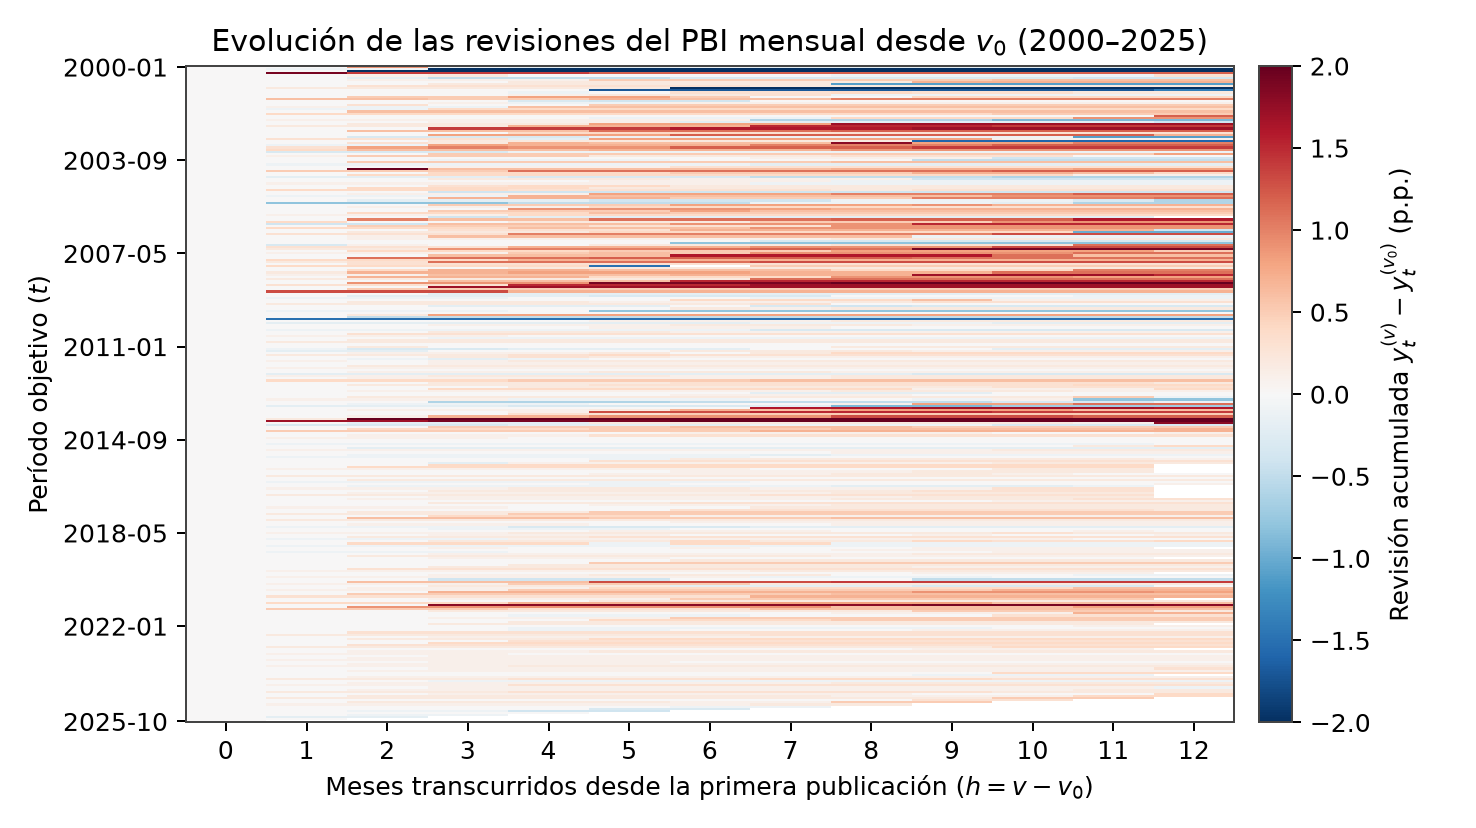
\includegraphics[width=0.92\textwidth]{images/triangulo_gdp.png}
	\caption{Evolución de las revisiones acumuladas del PBI mensual desde la primera publicación \(v_0\) (2000--2025)}
	\label{fig:triangulo}
	\fuente{elaboración propia a partir de los registros históricos del BCRP.}
\end{figure}

\subsection{Comportamiento básico de las revisiones}
\label{subsec:descriptivos}

El hallazgo principal al comparar cifras preliminares con sus versiones corregidas es directo: \textbf{cuando se publica por primera vez el PBI mensual del Perú, suele quedarse corto}. Como muestra la Tabla~\ref{tab:descriptivos_revision}, once meses después (\(H=11\)) la tasa corregida sube en promedio \(+0{,}347\) puntos porcentuales respecto al primer anuncio (y \(+0{,}363\) puntos si se mide a doce meses). La misma tendencia al alza aparece en todos los horizontes evaluados, desde tres meses (\(+0{,}205\) puntos) hasta la comparación con el último dato disponible (\(+0{,}256\) puntos, equivalente con signo invertido al \(-0{,}256\) visto en la lectura inicial; Anexo~\ref{app:objetivo}).

\begin{table}[htbp]
	\centering
	\caption{Estadísticos descriptivos de la revisión del PBI (\(y_t^{(v_H)} - y_t^{(v_0)}\)) según horizonte y depuración}
	\label{tab:descriptivos_revision}
	\footnotesize
	\setlength{\tabcolsep}{4.5pt}
	\renewcommand{\arraystretch}{1.15}
	\begin{tabular}{@{}l S[table-format=3.0] S[table-format=-1.3] S[table-format=1.3] S[table-format=-1.3] S[table-format=-1.3] S[table-format=-1.3] S[table-format=-1.3] S[table-format=1.3]@{}}
		\toprule
		Muestra / horizonte & {$n$} & {Media} & {DE} & {Mín.} & {P25} & {Mediana} & {P75} & {Máx.}\\
		\midrule
		\(H=11\) limpio (principal) & 350 & 0.347 & 0.768 & -2.000 & 0.000 & 0.200 & 0.600 & 4.900\\
		\(H=11\) bruto (con base) & 374 & 0.305 & 0.930 & -5.500 & 0.000 & 0.200 & 0.600 & 4.900\\
		\(H=12\) limpio (sensibilidad) & 331 & 0.363 & 0.798 & -2.000 & 0.000 & 0.200 & 0.700 & 4.900\\
		\(H=6\) limpio (sensibilidad) & 355 & 0.311 & 0.598 & -2.000 & 0.000 & 0.200 & 0.500 & 4.000\\
		\(H=3\) limpio (sensibilidad) & 358 & 0.205 & 0.452 & -1.500 & 0.000 & 0.100 & 0.300 & 2.500\\
		Horizonte variable (última \(-\) primera) & 406 & 0.256 & 0.930 & -5.500 & 0.000 & 0.200 & 0.600 & 4.200\\
		\bottomrule
	\end{tabular}
	\fuente{elaboración propia a partir de la muestra depurada de publicaciones del BCRP.}
\end{table}

La Tabla~\ref{tab:descriptivos_revision} también demuestra la utilidad de retirar los \(24\) meses afectados por cambios de año base: al separarlos, desaparece la caída extrema de \(-5{,}500\) puntos (quedando en \(-2{,}000\)) y la dispersión baja de \(0{,}930\) a \(0{,}768\), señal de que esos grandes saltos negativos reflejaban empalmes estadísticos y no correcciones corrientes. Por su parte, la demora habitual para publicar por primera vez un mes se mantuvo prácticamente fija en dos meses (promedio de \(2{,}003\) meses).

Las Figuras~\ref{fig:scatter}, \ref{fig:hist} y~\ref{fig:horizontes} ilustran visualmente estos rasgos: la relación casi uno a uno pero ligeramente desplazada hacia arriba entre primera y última cifra, la distribución concentrada a la derecha del cero tras separar cambios de base, y cómo cae la cantidad de datos útiles al alargar demasiado el horizonte (cayendo a \(5\) observaciones en \(18\) meses y a \(0\) en \(24\) meses).

\begin{figure}[htbp]
	\centering
	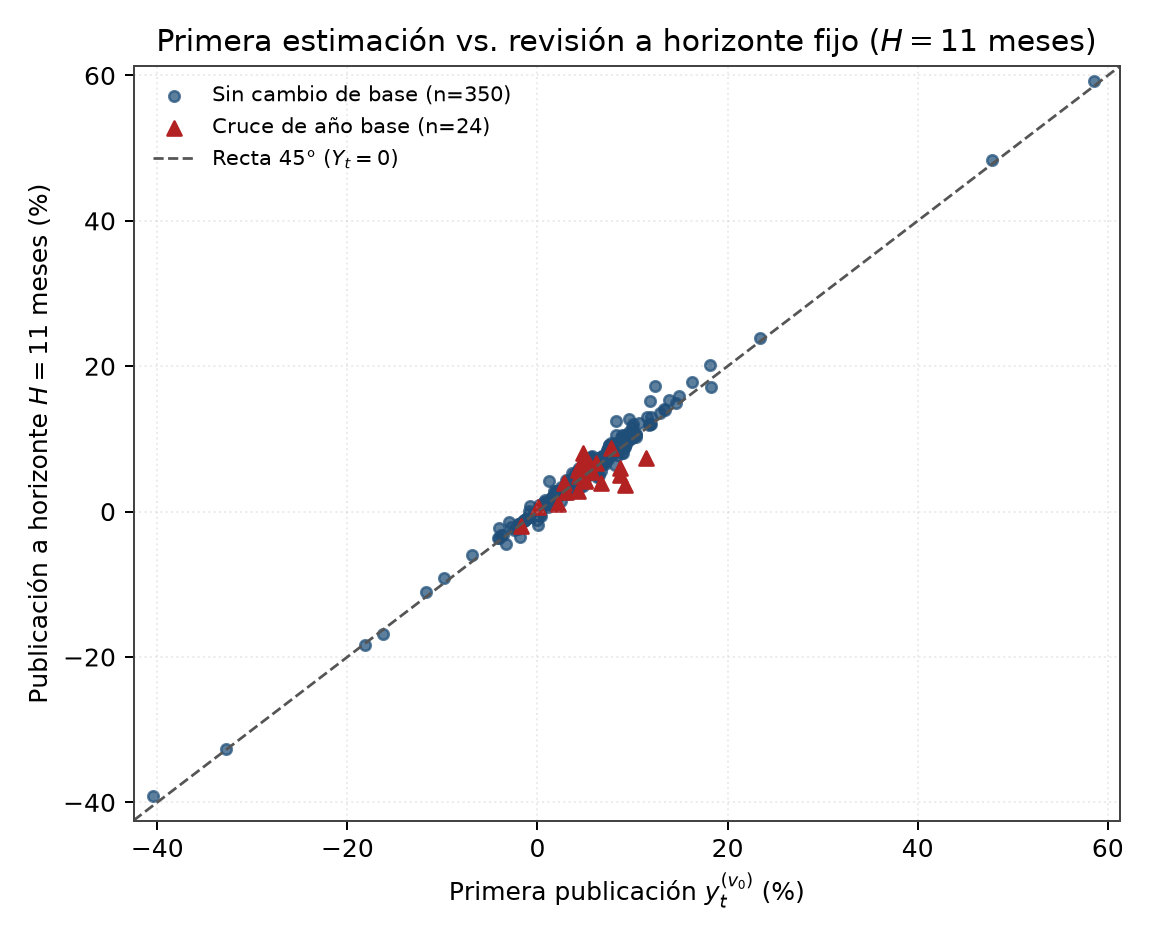
\includegraphics[width=0.72\textwidth]{images/scatter_revisiones_gdp.png}
	\caption{Primera publicación \(y_t^{(v_0)}\) frente a publicación a horizonte fijo \(H=11\) meses}
	\label{fig:scatter}
	\fuente{elaboración propia.}
\end{figure}

\begin{figure}[htbp]
	\centering
	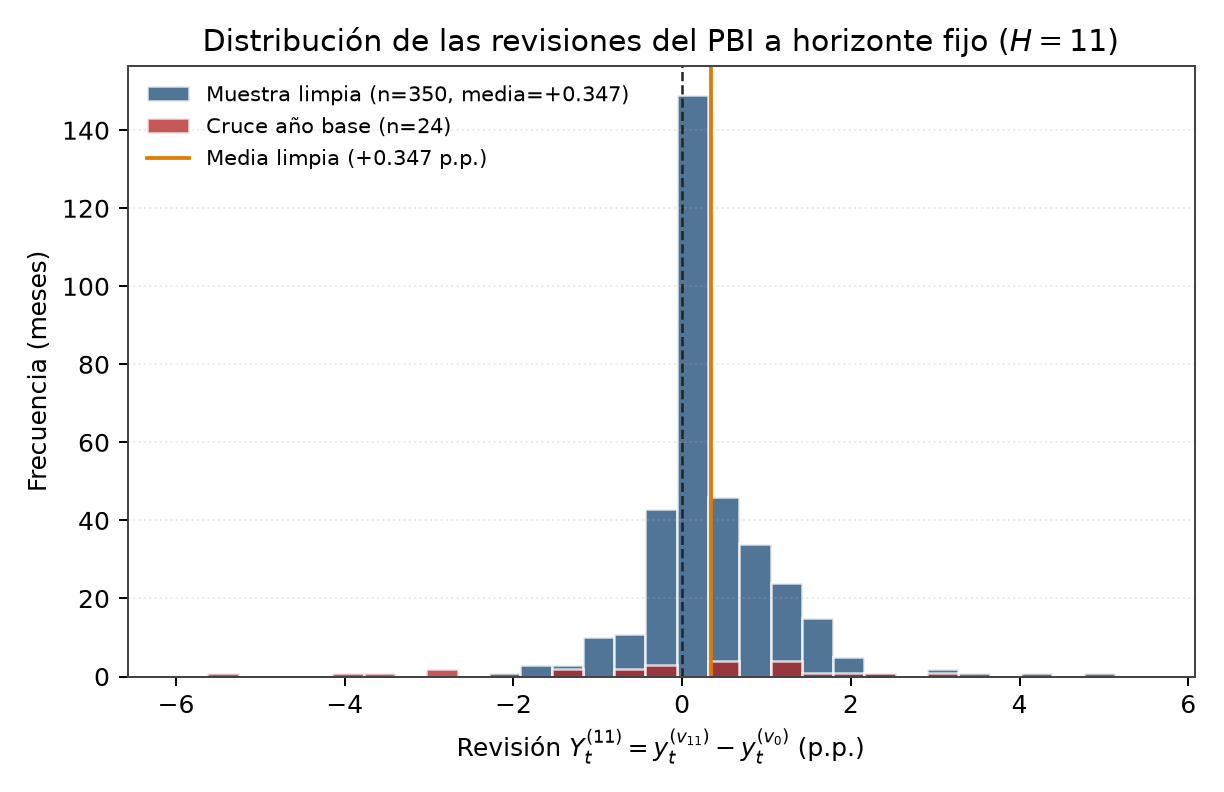
\includegraphics[width=0.76\textwidth]{images/hist_revisiones_gdp.png}
	\caption{Distribución de la revisión \(Y_t^{(11)} = y_t^{(v_{11})} - y_t^{(v_0)}\) con separación de cambios de año base}
	\label{fig:hist}
	\fuente{elaboración propia.}
\end{figure}

\begin{figure}[htbp]
	\centering
	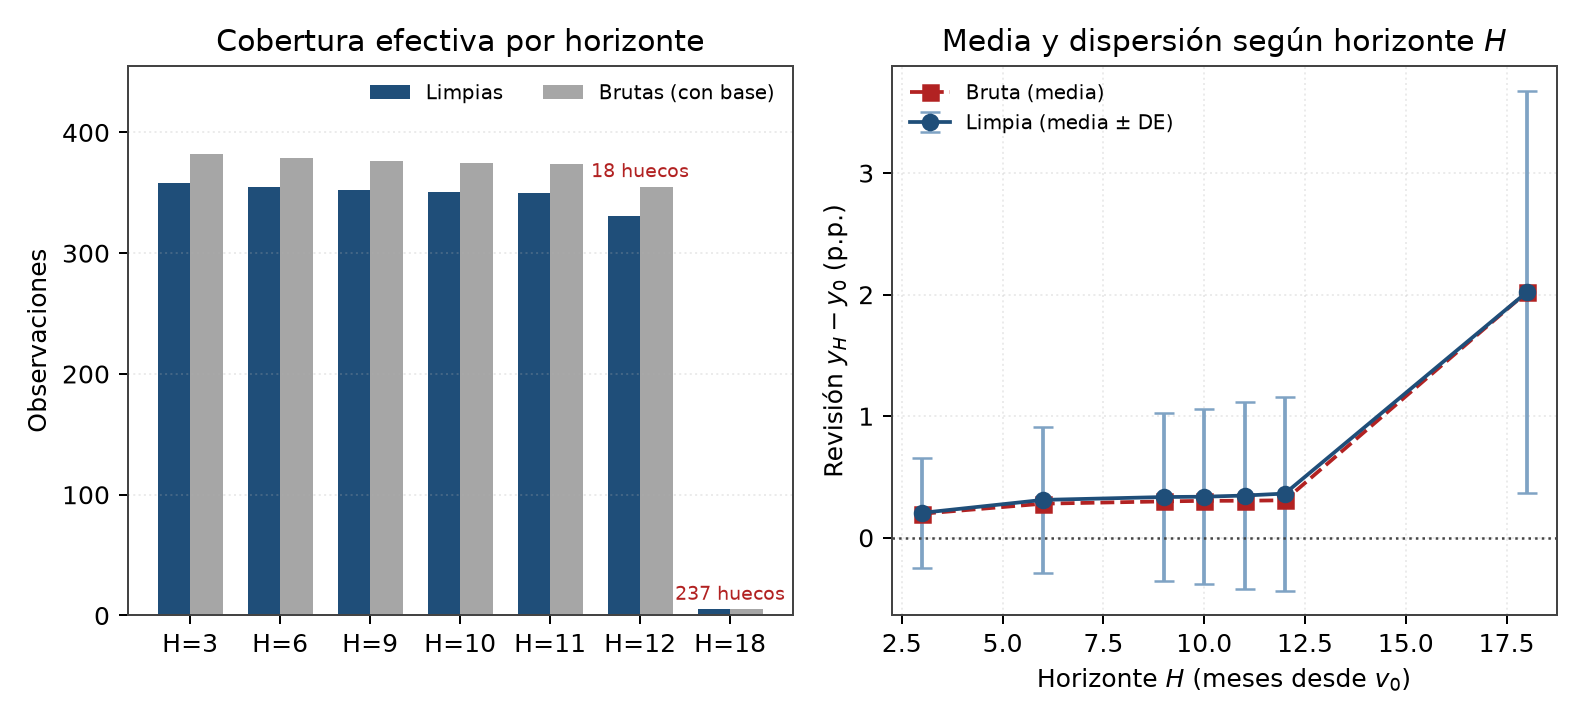
\includegraphics[width=0.92\textwidth]{images/metricas_horizonte_gdp.png}
	\caption{Cobertura efectiva y media/desviación estándar de las revisiones según horizonte \(H\)}
	\label{fig:horizontes}
	\fuente{elaboración propia.}
\end{figure}

\subsection{Qué patrones estadísticos siguen las revisiones}
\label{subsec:econometria}

Antes de entrenar modelos complejos, se verificó si las revisiones seguían reglas observables o si eran puro ruido. Las pruebas tomaron en cuenta que los errores de meses cercanos se parecen entre sí aplicando la corrección de \textcite{newey1987} (tanto en su versión estándar como considerando once meses de solapamiento).

\paragraph{Sesgo constante hacia arriba y valores extremos poco comunes.}
En todos los plazos evaluados (\(3\), \(6\), \(11\) y \(12\) meses), el promedio positivo es altamente significativo (\(p < 10^{-5}\); Tabla~\ref{tab:etapa2_sesgo}), descartando que se trate de coincidencia. Además, aparecen revisiones grandes positivas con más frecuencia de lo que tendría una campana normal (asimetría positiva y curtosis elevada, prueba de normalidad rechazada con \(p < 10^{-100}\)), razón por la cual las simulaciones posteriores incluyeron sacudidas no normales.

\begin{table}[htbp]
	\centering
	\caption{Pruebas estadísticas de sesgo medio y distribución en muestras limpias}
	\label{tab:etapa2_sesgo}
	\footnotesize
	\renewcommand{\arraystretch}{1.15}
	\begin{tabular}{@{}l S[table-format=3.0] S[table-format=1.3] S[table-format=1.3] l S[table-format=1.3] l S[table-format=1.3] S[table-format=1.3] S[table-format=3.1]@{}}
		\toprule
		Horizonte & {$n$} & {Media} & {$\text{SE}_{\text{NW}}$} & {\(p_{\text{NW}}\)} & {$\text{SE}_{\text{solap}}$} & {\(p_{\text{solap}}\)} & {Asim.} & {Curt.\ exc.} & {JB}\\
		\midrule
		\(H=3\)  & 358 & 0.205 & 0.033 & \(<10^{-9}\) & 0.031 & \(<10^{-10}\) & 1.394 & 5.736 & 589.4\\
		\(H=6\)  & 355 & 0.311 & 0.047 & \(<10^{-10}\) & 0.049 & \(<10^{-9}\)  & 1.163 & 6.523 & 687.9\\
		\(H=11\) & 350 & 0.347 & 0.064 & \(5{,}3\times 10^{-8}\) & 0.075 & \(3{,}6\times 10^{-6}\) & 1.258 & 6.293 & 649.6\\
		\(H=12\) & 331 & 0.363 & 0.067 & \(5{,}7\times 10^{-8}\) & 0.080 & \(5{,}6\times 10^{-6}\) & 1.145 & 5.465 & 468.6\\
		\bottomrule
	\end{tabular}
	\fuente{elaboración propia a partir de las pruebas econométricas sobre la muestra depurada. Todos los estadísticos Jarque--Bera arrojan \(p < 10^{-100}\).}
\end{table}

\paragraph{Un ciclo anual repetitivo y diferencias por mes.}
La Figura~\ref{fig:acf_estac} revela un detalle práctico clave para pronosticar en tiempo real: aunque las revisiones de meses inmediatos están fuertemente conectadas entre sí (\(\hat{\rho}_1 = +0{,}453\); \cite{ljung1978} \(p = 1{,}4\times 10^{-41}\)), esas revisiones recientes todavía no terminan cuando nace un dato nuevo. En cambio, las revisiones que sí ya terminaron \textbf{un año atrás} conservan una relación clara con el mes actual (correlación anual de \(+0{,}386\) en el mes doce, \(p=1{,}3\times 10^{-12}\)). A esto se suma un patrón estacional marcado: el primer trimestre del año recibe las mayores correcciones hacia arriba (enero \(+0{,}731\), febrero \(+0{,}503\) y marzo \(+0{,}734\) puntos), mientras noviembre (\(+0{,}143\)) y diciembre (\(-0{,}083\)) apenas cambian.

\begin{figure}[htbp]
	\centering
	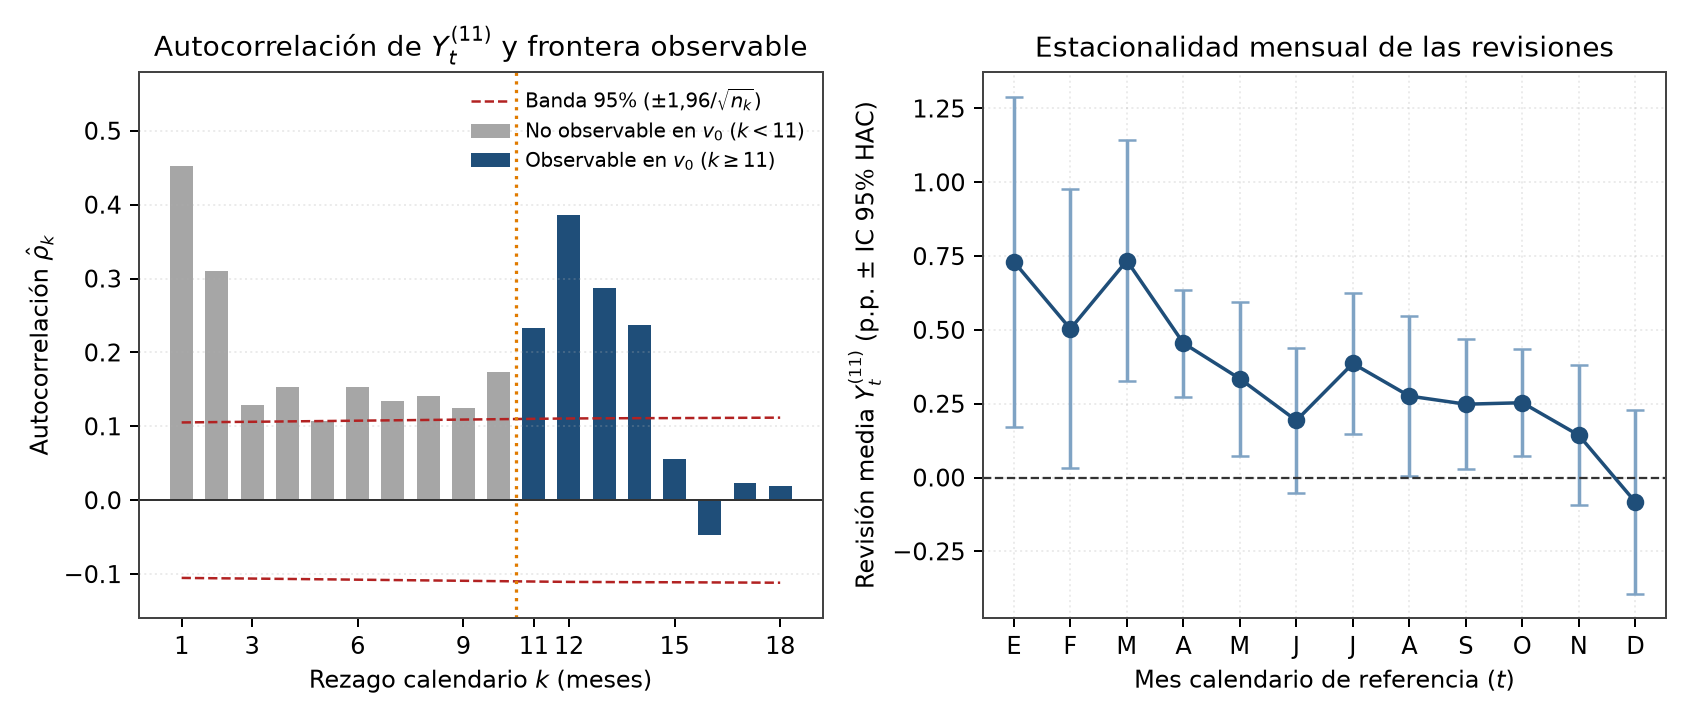
\includegraphics[width=0.95\textwidth]{images/etapa2_acf_pacf.png}
	\caption{Repetición temporal de la revisión \(Y_t^{(11)}\) respecto a la frontera observable en tiempo real (izquierda) y promedio por mes del año (derecha)}
	\label{fig:acf_estac}
	\fuente{elaboración propia a partir de la serie histórica limpia (\(n=350\)).}
\end{figure}

La Tabla~\ref{tab:etapa2_rt} comprueba cuánta variación de las revisiones se explica usando únicamente información ya disponible en el primer anuncio (\(n=313\)). Los dos rezagos anuales completados explican por sí solos un \(15{,}7\%\) (\(R^2 = 0{,}1569\)), y al juntarlos con el dato preliminar, cambios recientes ya publicados y el mes del año se alcanza un \(22{,}3\%\) (\(R^2 = 0{,}2225\), \(p = 2{,}6\times 10^{-7}\)). Este resultado confirma la Hipótesis~1: las revisiones del PBI tienen una señal real predecible.

\begin{table}[htbp]
	\centering
	\caption{Capacidad explicativa usando únicamente información observable en \(v_0(t)\) (\(n=313\))}
	\label{tab:etapa2_rt}
	\footnotesize
	\renewcommand{\arraystretch}{1.15}
	\begin{tabular}{@{}l c S[table-format=1.4] S[table-format=1.4] S[table-format=1.3] l S[table-format=3.2]@{}}
		\toprule
		Información observable en \(v_0(t)\) & Variables & {\(R^2\)} & {\(\bar{R}^2\)} & {\(F_{\text{NW}}\)} & {\(p\)-valor HAC} & {BIC}\\
		\midrule
		Solo primera publicación (\(y_t^{(v_0)}\)) & 1 & 0.0230 & 0.0198 & 4.999 & \(0{,}0261\) & 677.59\\
		Revisiones de hace 1 año (\(Y_{t-11}, Y_{t-12}\)) & 2 & 0.1569 & 0.1515 & 9.197 & \(1{,}3\times 10^{-4}\) & 637.20\\
		Revisiones recientes observables (\(s=1,2\)) & 2 & 0.0179 & 0.0115 & 4.120 & \(0{,}0171\) & 684.97\\
		Mes del año (estacionalidad) & 11 & 0.0807 & 0.0471 & 2.249 & \(0{,}0122\) & 716.00\\
		Modelo conjunto observable en \(v_0\) & 16 & 0.2225 & 0.1804 & 4.190 & \(2{,}6\times 10^{-7}\) & 692.30\\
		\bottomrule
	\end{tabular}
	\fuente{elaboración propia con base en las estimaciones en tiempo real del estudio.}
\end{table}

\paragraph{Estabilidad por épocas, efecto de la pandemia y diferencias entre sectores.}
Al comprobar mediante la prueba de \textcite{mincer1969} si la primera cifra refleja toda la información sin sesgo (Tabla~\ref{tab:etapa2_mz}), en todas las épocas se rechaza la eficiencia perfecta debido principalmente al empuje constante hacia arriba (\(\hat{\alpha} > 0\)). Al revisar qué cambió con los años (Figura~\ref{fig:regimenes}), sobresalen dos hechos muy importantes:
\begin{enumerate}
	\item \textbf{La variabilidad bajó antes de la pandemia:} entre 1993 y 2012 las revisiones oscilaban bastante (desviación estándar de \(1{,}289\) y \(0{,}716\)), pero entre 2014 y 2019 la serie se volvió muy estable (\(\text{DE}=0{,}196\)), aunque mantuvo su sesgo positivo de \(+0{,}163\) puntos \parencite{engle1982}.
	\item \textbf{Las relaciones curvas aparecen solo por la pandemia:} aunque la prueba de linealidad de \textcite{ramsey1969} marca señal no lineal en la serie completa (\(p=0{,}0010\)), al mirar época por época se descubre que antes de 2020 una relación recta funcionaba perfectamente bien (2000--2012 \(p=0{,}9112\); 2014--2019 \(p=0{,}2085\)). La curvatura aparece únicamente entre 2020 y 2024 (\(p=0{,}0003\)), motivando analizar los modelos antes y después del COVID-19 por separado.
\end{enumerate}

\begin{table}[htbp]
	\centering
	\caption{Pruebas de eficiencia (\(y_t^{(v_H)} = \alpha + \beta y_t^{(v_0)} + u_t\)) y diagnósticos por época}
	\label{tab:etapa2_mz}
	\footnotesize
	\setlength{\tabcolsep}{4pt}
	\renewcommand{\arraystretch}{1.15}
	\begin{tabular}{@{}l S[table-format=3.0] S[table-format=1.3] S[table-format=1.3] S[table-format=1.3] S[table-format=1.3] S[table-format=2.2] l l l@{}}
		\toprule
		Muestra / época & {$n$} & {\(\hat{\alpha}\)} & {\(\text{SE}_{\alpha}\)} & {\(\hat{\beta}\)} & {\(\text{SE}_{\beta}\)} & {\(F_{\text{Wald}}\)} & {\(p_{\text{Wald}}\)} & {\(p_{\text{ARCH}}\)} & {\(p_{\text{RESET}}\)}\\
		\midrule
		Limpia \(H=11\) (global) & 350 & 0.273 & 0.064 & 1.018 & 0.010 & 16.23 & \(1{,}8\times 10^{-7}\) & \(3{,}1\times 10^{-7}\) & \(0{,}0010\)\\
		Limpia \(H=12\) (global) & 331 & 0.297 & 0.067 & 1.016 & 0.009 & 15.84 & \(2{,}7\times 10^{-7}\) & \(1{,}2\times 10^{-6}\) & \(0{,}0048\)\\
		Limpia \(H=6\) (global)  & 355 & 0.270 & 0.051 & 1.010 & 0.007 & 23.35 & \(3{,}0\times 10^{-10}\) & \(5{,}5\times 10^{-6}\) & \(0{,}0038\)\\
		Limpia \(H=3\) (global)  & 358 & 0.172 & 0.032 & 1.008 & 0.005 & 20.70 & \(3{,}1\times 10^{-9}\) & \(9{,}6\times 10^{-6}\) & \(0{,}1283\)\\
		\midrule
		1993-10 a 1999-04 (Base 90/94) & 67 & 0.356 & 0.245 & 1.052 & 0.041 & 4.69 & \(0{,}0125\) & \(0{,}4572\) & \(0{,}0514\)\\
		2000-06 a 2012-12 (Base 94)    & 151 & 0.054 & 0.129 & 1.052 & 0.022 & 10.42 & \(5{,}8\times 10^{-5}\) & \(0{,}0407\) & \(0{,}9112\)\\
		2014-02 a 2019-12 (Pre-COVID)  & 71 & 0.180 & 0.047 & 0.994 & 0.012 & 16.96 & \(1{,}0\times 10^{-6}\) & \(0{,}0231\) & \(0{,}2085\)\\
		2020-01 a 2024-11 (COVID+)     & 59 & 0.297 & 0.057 & 1.004 & 0.006 & 13.95 & \(1{,}2\times 10^{-5}\) & \(0{,}5904\) & \(0{,}0003\)\\
		\bottomrule
	\end{tabular}
	\fuente{elaboración propia con ajuste de errores estándar HAC (\(L_{\text{NW}}\)).}
\end{table}

\begin{figure}[htbp]
	\centering
	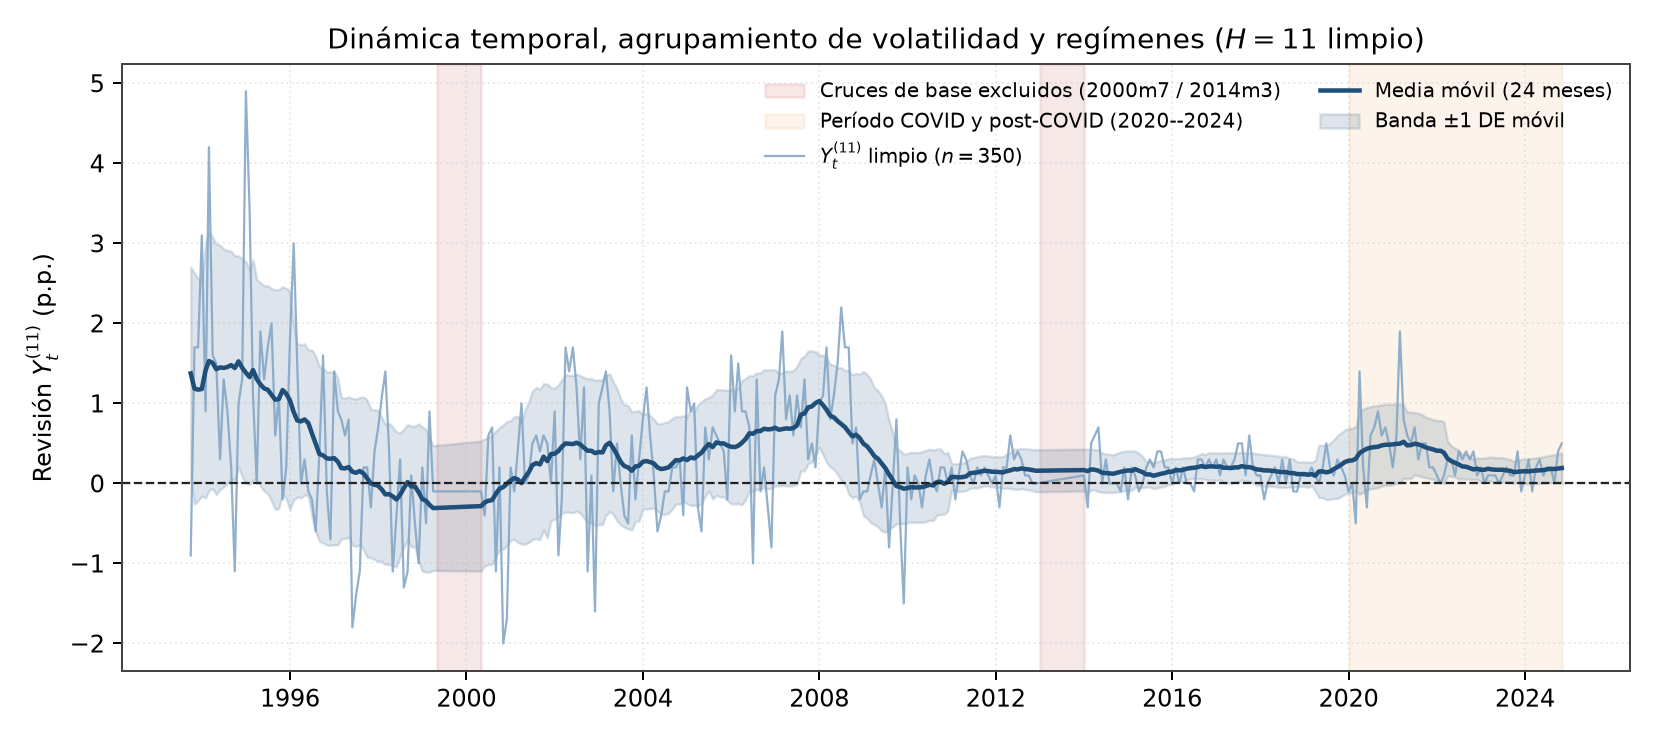
\includegraphics[width=0.95\textwidth]{images/etapa2_regimenes_evolucion.png}
	\caption{Evolución temporal de \(Y_t^{(11)}\), promedio y dispersión móviles por épocas económicas (1993--2024)}
	\label{fig:regimenes}
	\fuente{elaboración propia a partir de la serie limpia del PBI peruano.}
\end{figure}

Por último, la Figura~\ref{fig:sectores} muestra que las correcciones al alza no ocurren por igual en toda la economía: se concentran en pesca (\(+2{,}143\) puntos), agropecuario (\(+0{,}821\)), comercio (\(+0{,}562\)), manufactura (\(+0{,}525\)) y minería (\(+0{,}505\)), sectores donde es más difícil reunir cifras completas el primer mes. En cambio, construcción (\(+0{,}098\)), servicios (\(+0{,}076\)) y electricidad (\(-0{,}011\)) casi no se corrigen en promedio.

\begin{figure}[htbp]
	\centering
	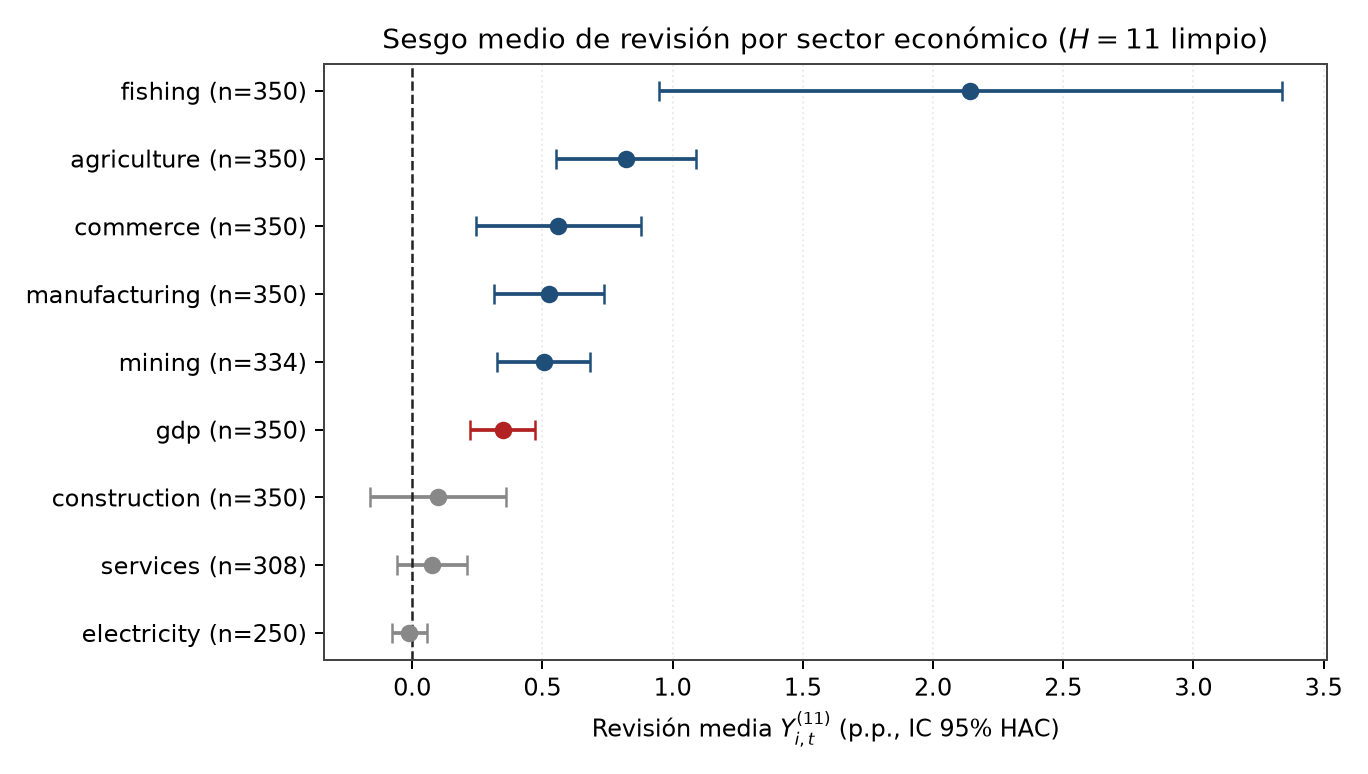
\includegraphics[width=0.82\textwidth]{images/etapa2_sectores_sesgo.png}
	\caption{Sesgo medio de revisión por sector económico a horizonte \(H=11\) limpio (intervalo de confianza al 95\%)}
	\label{fig:sectores}
	\fuente{elaboración propia con base en las series sectoriales verificadas.}
\end{figure}

\subsection{Desempeño de los modelos prediciendo mes a mes}
\label{subsec:desempeno_modelos}

Para probar qué modelo predice mejor en condiciones reales, los doce competidores emitieron pronósticos mes a mes durante más de veinte años: \(250\) fechas entre febrero de 2003 y noviembre de 2024. En cada mes solo se entrenaron con el historial ya cerrado hasta ese día, manteniendo aparte los últimos \(60\) meses (diciembre de 2019 a noviembre de 2024) para el examen final. De forma automática dentro del pasado, el modelo autorregresivo eligió casi siempre mirar los dos años anteriores (\(99{,}2\%\) de las veces) y Ridge aplicó una regularización alta (\(\lambda=500\)) para equilibrar las variables sectoriales.

La Tabla~\ref{tab:metricas} resume los errores globales de todo el período, y la Tabla~\ref{tab:etapa3_regimenes} separa lo ocurrido antes de la pandemia y durante los últimos cinco años. En la lectura global, \textbf{el menor error correspondió a las características aleatorias de Fourier (RFF, \(\text{RMSE}=0{,}456\))}, seguidas por la red clásica ESN de veinte neuronas (\(\text{RMSE}=0{,}472\)) y recién en tercer lugar por el modelo cuántico QRC (\(\text{RMSE}=0{,}478\)).

\begin{table}[htbp]
	\centering
	\caption{Desempeño predictivo global de los doce modelos sobre \(Y_t^{(11)}\) (2003m2--2024m11, \(n=250\))}
	\label{tab:metricas}
	\footnotesize
	\renewcommand{\arraystretch}{1.15}
	\begin{tabular}{@{}>{\raggedright\arraybackslash}p{4.5cm}S[table-format=1.3]S[table-format=1.3]S[table-format=-1.3]S[table-format=-1.3]l@{}}
		\toprule
		Modelo & {RMSE} & {MAE} & {Sesgo} & {$R^2_{\text{OOS}}$} & {IC 95\% \(\Delta\text{RMSE}\) (vs. Ridge)}\\
		\midrule
		Referencia nula (\(\widehat{Y}=0\)) & 0.574 & 0.396 & 0.292 & -0.349 & {\([-0{,}135;\; +0{,}150]\), \(p_{\text{DM}}=0{,}918\)}\\
		Corrección de sesgo (media exp.) & 0.513 & 0.395 & -0.131 & -0.077 & {\([-0{,}176;\; +0{,}057]\), \(p_{\text{DM}}=0{,}430\)}\\
		Corrección de sesgo (móvil 60m) & 0.525 & 0.381 & 0.021 & -0.127 & {\([-0{,}164;\; +0{,}064]\), \(p_{\text{DM}}=0{,}512\)}\\
		Autorregresivo AR (BIC) & 0.498 & 0.356 & -0.037 & -0.016 & {\([-0{,}189;\; +0{,}044]\), \(p_{\text{DM}}=0{,}301\)}\\
		ARX observable (BIC) & 0.558 & 0.384 & -0.015 & -0.276 & {\([-0{,}068;\; +0{,}037]\), \(p_{\text{DM}}=0{,}791\)}\\
		Regresión Ridge (benchmark, 20 var.) & 0.566 & 0.384 & -0.064 & -0.312 & {Referencia principal (\(0{,}000\))}\\
		Factores dinámicos (DFM + Ridge) & 0.605 & 0.392 & -0.067 & -0.498 & {\([-0{,}001;\; +0{,}086]\), \(p_{\text{DM}}=0{,}184\)}\\
		Árboles potenciados (GBDT)\textsuperscript{a} & 0.495 & 0.356 & -0.068 & -0.003 & {\([-0{,}193;\; +0{,}032]\), \(p_{\text{DM}}=0{,}290\)}\\
		Características aleatorias (RFF, \(m=20\))\textsuperscript{b} & 0.456 & 0.334 & -0.069 & 0.149 & {\([-0{,}222;\; -0{,}013]\), \(p_{\text{DM}}=0{,}094\)}\\
		Reservorio clásico ESN (20 n.)\textsuperscript{b} & 0.472 & 0.341 & -0.057 & 0.087 & {\([-0{,}188;\; -0{,}004]\), \(p_{\text{DM}}=0{,}103\)}\\
		Reservorio clásico ESN (64 n.)\textsuperscript{b} & 0.508 & 0.379 & -0.038 & -0.056 & {\([-0{,}136;\; +0{,}014]\), \(p_{\text{DM}}=0{,}200\)}\\
		Reservorio cuántico QRC (5 qubits)\textsuperscript{b} & 0.478 & 0.352 & -0.102 & 0.063 & {\([-0{,}208;\; +0{,}020]\), \(p_{\text{DM}}=0{,}196\)}\\
		\bottomrule
	\end{tabular}
	\caption*{\footnotesize \textit{Nota:} \textsuperscript{a}Árboles CART acotados (\texttt{GBDT\_NumPy} en gráficos). \textsuperscript{b}Promedios deterministas sobre cinco semillas (\texttt{101, 202, 303, 404, 505}); \texttt{QRC\_Ising5} usa simulación exacta por matriz densidad. Intervalos bootstrap por bloques \parencite{politis1992} (\(L=12\), \(B=2000\)); valor \(p_{\text{DM}}\) bilateral de \textcite{harvey1997}.}
	\fuente{elaboración propia con base en las evaluaciones fuera de muestra del estudio (2003--2024).}
\end{table}

Al separar los períodos normales de la pandemia en la Tabla~\ref{tab:etapa3_regimenes} (y las Figuras~\ref{fig:etapa3_oos}--\ref{fig:etapa4_estabilidad}), la historia queda completamente clara:
\begin{enumerate}
	\item \textbf{En épocas normales (2003--2019), la regresión Ridge funcionó bien:} antes del COVID-19, Ridge fue el mejor modelo lineal clásico (\(\text{RMSE}=0{,}503\)), superando con claridad al promedio histórico simple (\(0{,}550\), \(p=0{,}0071\)) y a los árboles de decisión (\(0{,}533\), \(p=0{,}0086\)). Incluso entre 2014 y 2019 el simple promedio móvil de sesenta meses logró \(\text{RMSE}=0{,}210\) con sesgo casi nulo.
	\item \textbf{Durante la pandemia (2020--2024), las fórmulas lineales se dispararon y los modelos acotados evitaron el error:} en abril de 2020 la primera cifra del PBI cayó \(-40{,}5\%\) y en abril de 2021 rebotó \(+58{,}5\%\). Al aplicar una recta sobre números tan extremos, Ridge predijo correcciones absurdas (\(-1{,}464\) y \(+4{,}020\) puntos porcentuales, cuando la revisión real fue \(+1{,}4\) y \(+0{,}8\)), elevando su error a \(\text{RMSE}=0{,}731\). Eso también distorsionó la prueba anidada de \textcite{clark2007} (\(\text{CW}=3{,}554\)). En cambio, los \textbf{árboles acotados (GBDT)} limitaron sus pronósticos (\(+0{,}241\) y \(+0{,}909\)) y obtuvieron el mejor desempeño del tramo final (\(\text{RMSE}=0{,}349\)), superando tanto a Ridge como a la referencia nula.
	\item \textbf{El modelo cuántico (QRC) frenó los extremos, pero no venció a los equivalentes clásicos:} gracias a que sus veinte mediciones quedan acotadas entre \(-1\) y \(+1\), QRC logró el segundo mejor error en pandemia (\(\text{RMSE}=0{,}363\)) y superó globalmente a la simple corrección por promedio histórico (\(0{,}478\) vs. \(0{,}513\), \(p=0{,}0175\)). Sin embargo, no venció a sus controles clásicos equivalentes: empató estadísticamente con ESN de veinte neuronas (\(0{,}472\), \(p=0{,}730\)) y perdió frente a RFF (\(0{,}456\), \(p=0{,}0146\) global y \(p=0{,}0038\) antes de la pandemia). Además, aumentar ESN de \(20\) a \(64\) neuronas empeoró el resultado (\(0{,}508\), \(p=0{,}046\)), probando que las series económicas cortas premian modelos compactos. También se observó que QRC varía bastante según la semilla aleatoria usada (promedio individual \(0{,}5160 \pm 0{,}0316\)), por lo que su resultado final dependió de promediar cinco ejecuciones.
\end{enumerate}

\begin{table}[htbp]
	\centering
	\caption{Desempeño antes del COVID-19 (2003m2--2019m11) frente al tramo final congelado (2019m12--2024m11)}
	\label{tab:etapa3_regimenes}
	\footnotesize
	\renewcommand{\arraystretch}{1.12}
	\begin{tabular}{@{}>{\raggedright\arraybackslash}p{4.5cm}S[table-format=1.3]S[table-format=1.3]S[table-format=-1.3]S[table-format=1.3]S[table-format=1.3]S[table-format=-1.3]@{}}
		\toprule
		& \multicolumn{3}{c}{Pre-pandemia (\(n=190\))} & \multicolumn{3}{c}{Tramo final (\(n=60\))}\\
		\cmidrule(lr){2-4}\cmidrule(lr){5-7}
		Modelo & {RMSE} & {MAE} & {$R^2_{\text{OOS}}$} & {RMSE} & {MAE} & {$R^2_{\text{OOS}}$}\\
		\midrule
		Referencia nula (\(\widehat{Y}=0\)) & 0.602 & 0.414 & -0.299 & 0.474 & 0.338 & -0.682\\
		Corrección media expansiva & 0.550 & 0.433 & -0.084 & 0.371 & 0.274 & -0.033\\
		Corrección móvil \(60\text{m}\) & 0.559 & 0.416 & -0.120 & 0.396 & 0.269 & -0.175\\
		Autorregresivo AR (BIC) & 0.526 & 0.384 & 0.007 & 0.396 & 0.267 & -0.175\\
		ARX observable (BIC) & 0.521 & 0.383 & 0.028 & 0.663 & 0.387 & -2.290\\
		Regresión Ridge (benchmark) & 0.503 & 0.375 & 0.094 & 0.731 & 0.413 & -3.001\\
		Factores dinámicos (DFM + Ridge) & 0.515 & 0.379 & 0.050 & 0.827 & 0.434 & -4.125\\
		Árboles potenciados (GBDT) & 0.533 & 0.394 & -0.017 & 0.349 & 0.237 & 0.087\\
		Características aleatorias (RFF) & 0.480 & 0.355 & 0.174 & 0.368 & 0.269 & -0.017\\
		Reservorio clásico ESN (20 n.) & 0.485 & 0.359 & 0.156 & 0.427 & 0.285 & -0.367\\
		Reservorio clásico ESN (64 n.) & 0.505 & 0.389 & 0.088 & 0.518 & 0.348 & -1.008\\
		Reservorio cuántico QRC (5 qubits) & 0.509 & 0.379 & 0.070 & 0.363 & 0.266 & 0.013\\
		\bottomrule
	\end{tabular}
	\fuente{elaboración propia con base en los resultados fuera de muestra por épocas (2003--2024).}
\end{table}

En síntesis, la capacidad de contener choques como los de 2020--2021 provino simplemente del acotamiento no lineal de las variables, y no de una ventaja propia de la mecánica cuántica (las pruebas numéricas previas confirmaron asimismo fidelidad física exacta del simulador, con errores inferiores a \(10^{-14}\), y cero uso de datos futuros).

\begin{figure}[htbp]
	\centering
	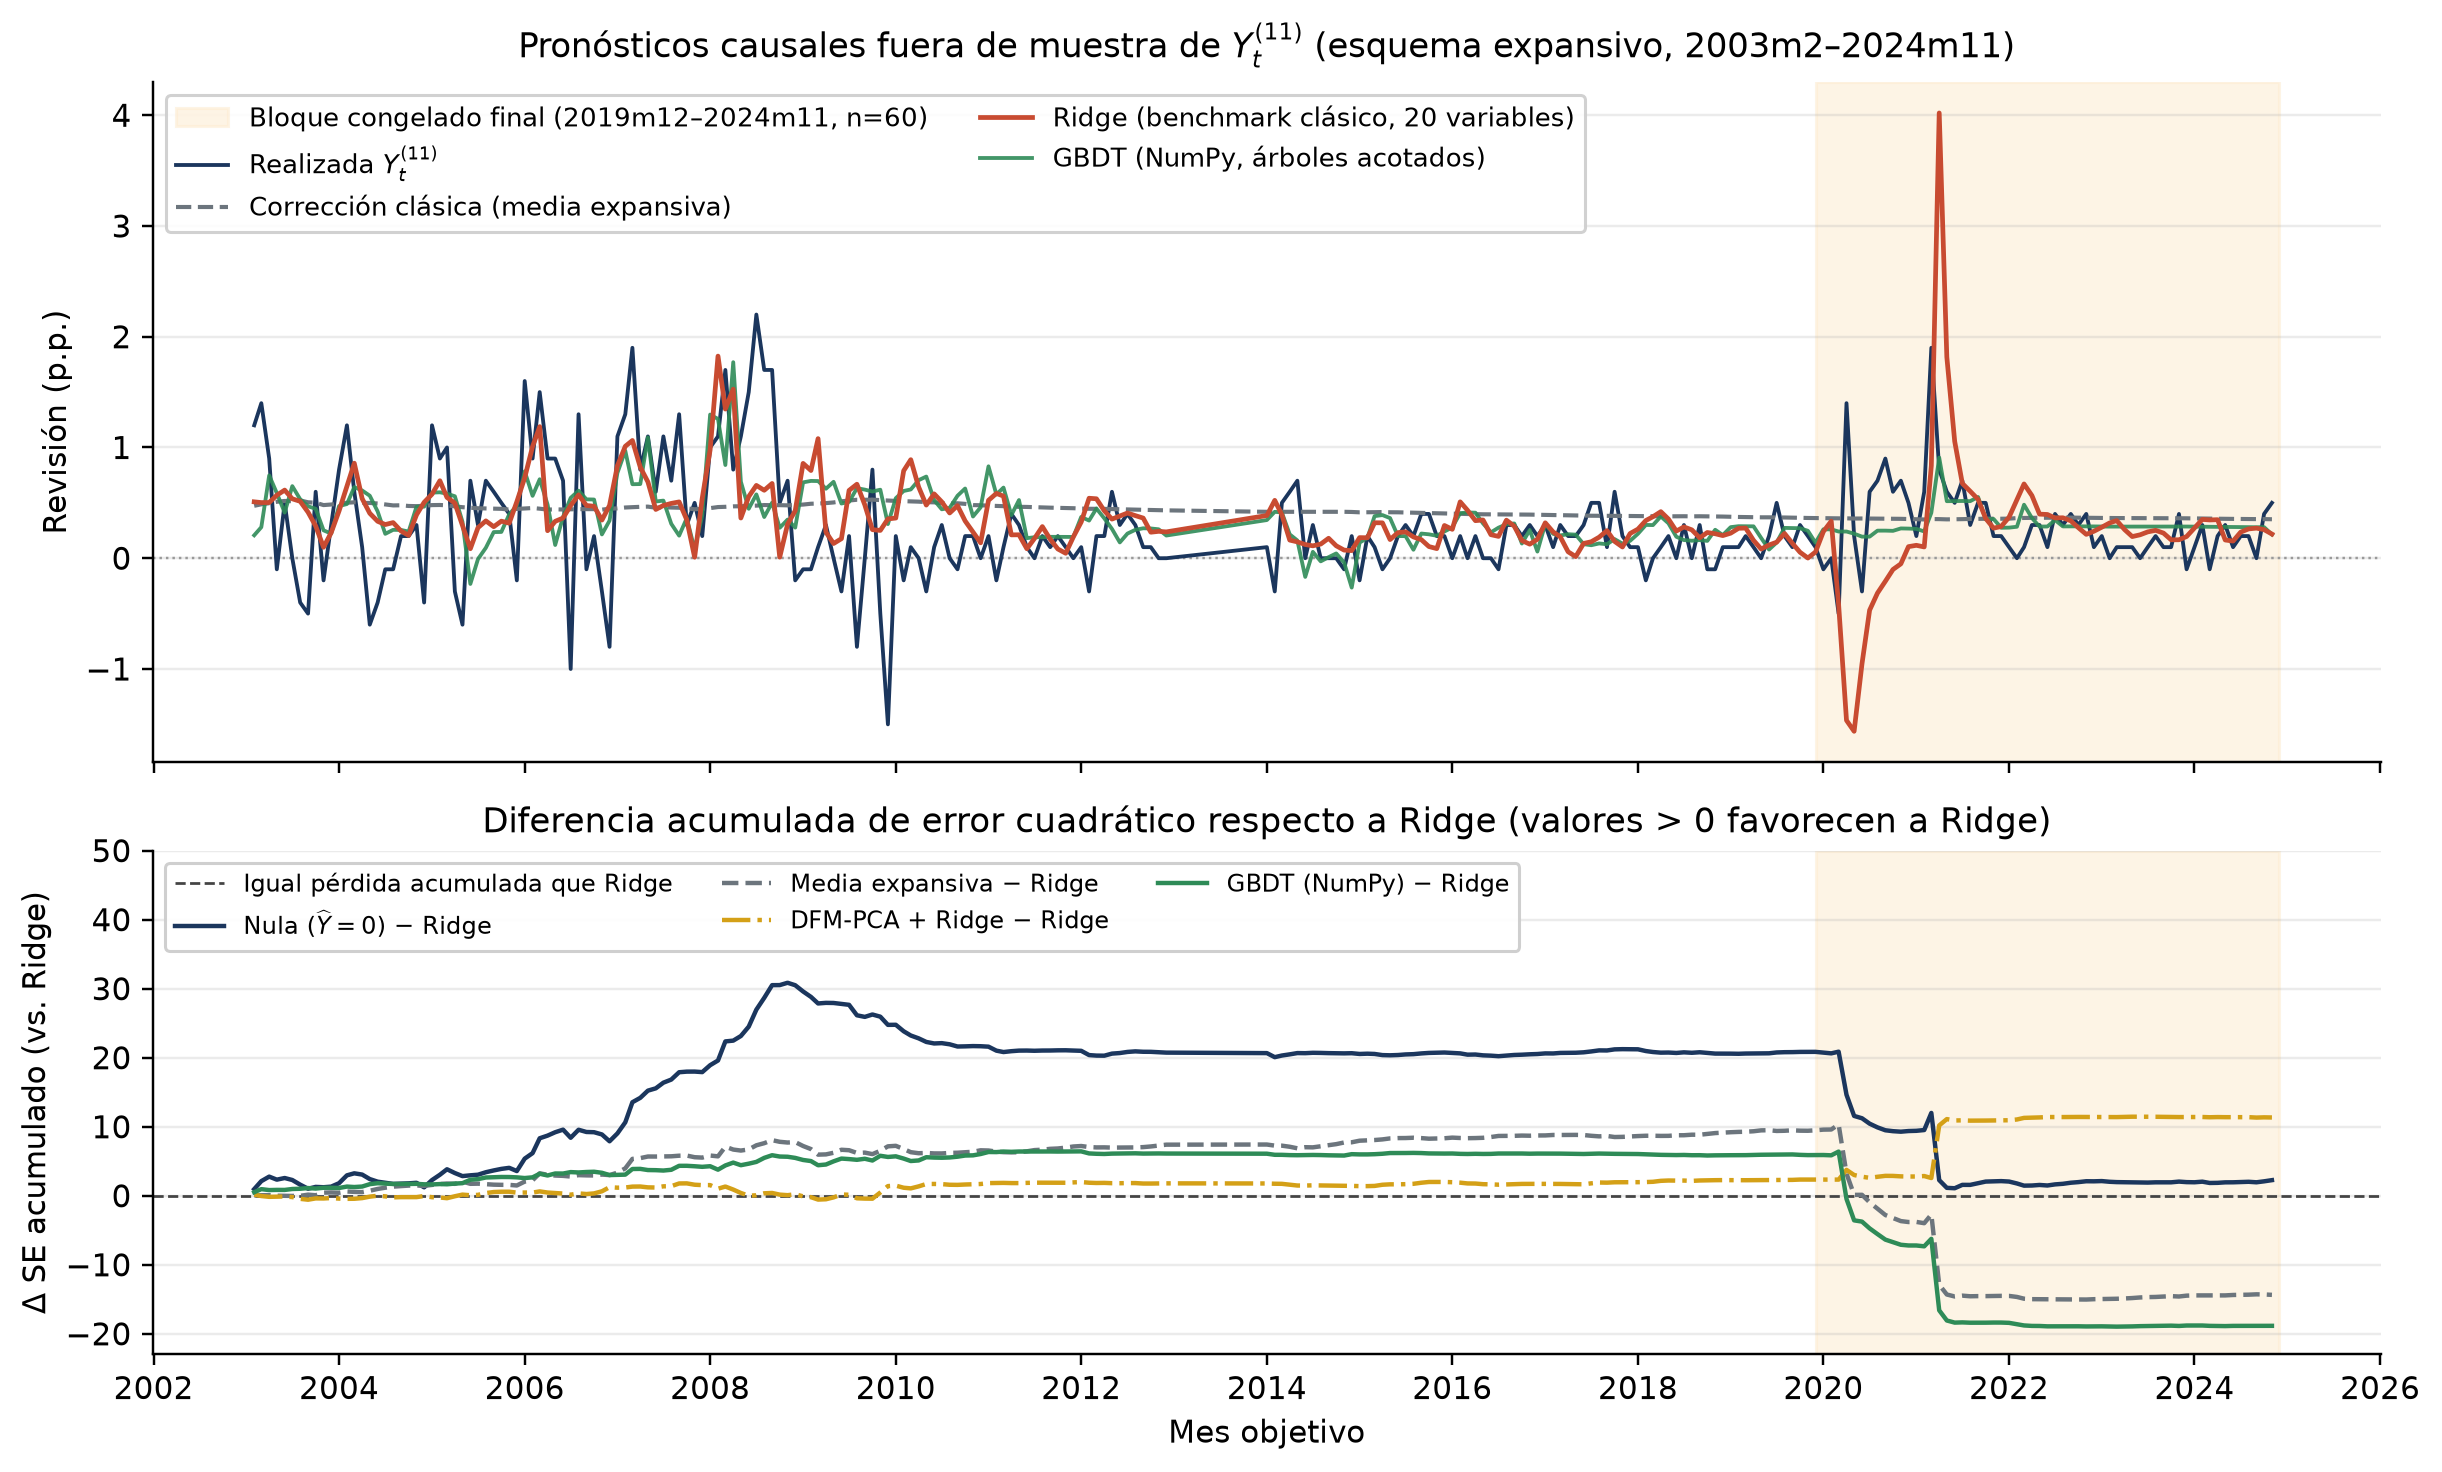
\includegraphics[width=0.96\textwidth]{images/etapa3_oos_predicciones.png}
	\caption{Pronósticos mensuales en tiempo real de modelos clásicos (arriba) y error acumulado frente a Ridge (abajo), 2003m2--2024m11.}
	\label{fig:etapa3_oos}
\end{figure}

\begin{figure}[htbp]
	\centering
	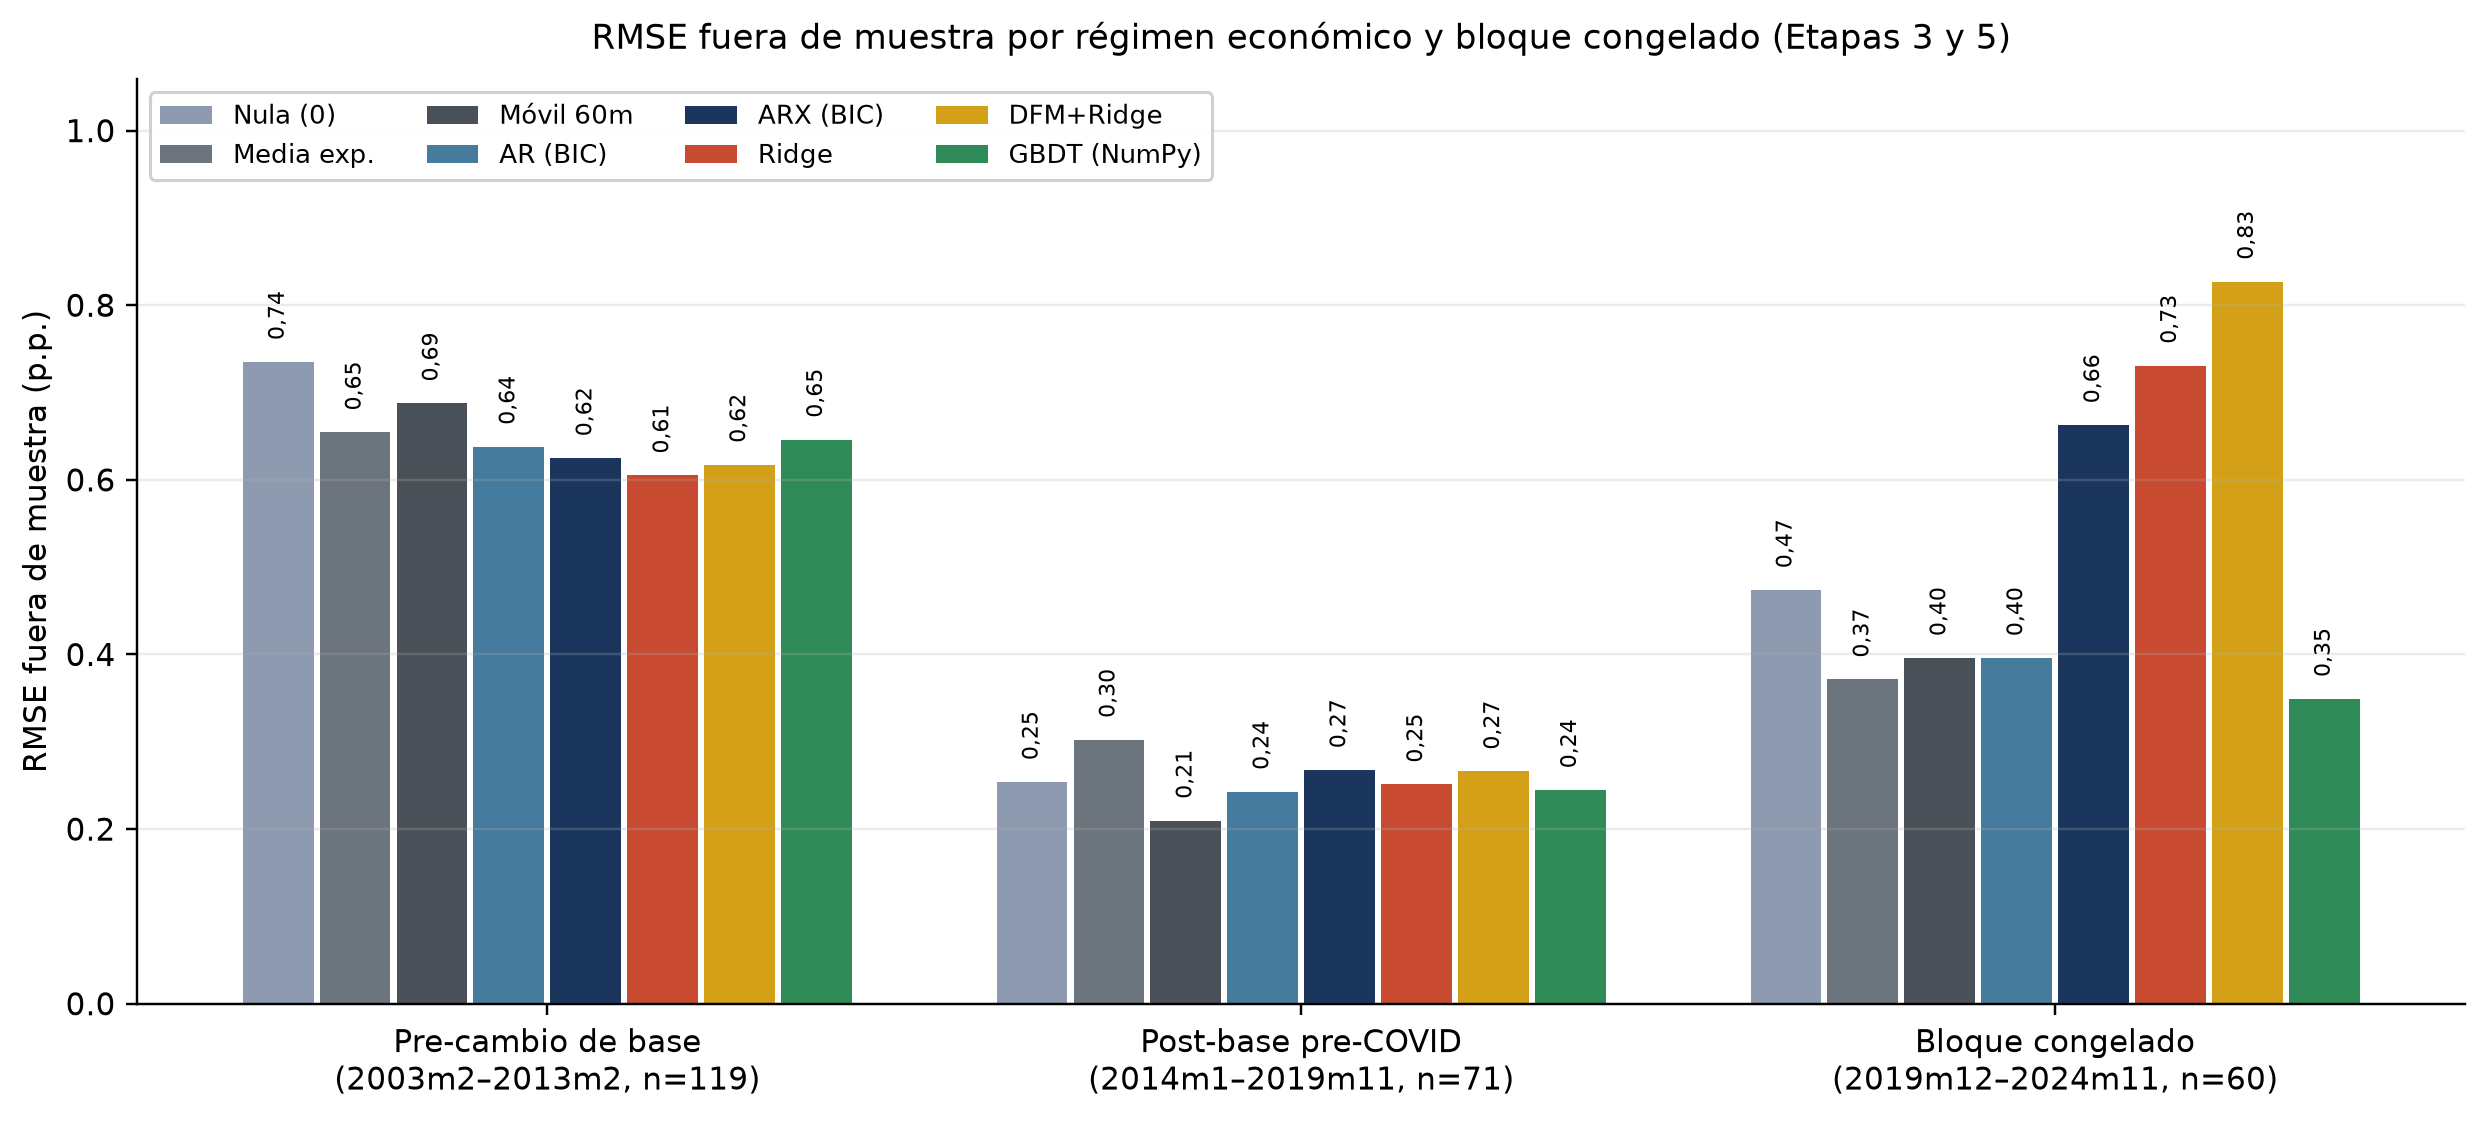
\includegraphics[width=0.96\textwidth]{images/etapa3_rmse_regimenes.png}
	\caption{Error RMSE por época económica y tramo final para los ocho referentes clásicos.}
	\label{fig:etapa3_regimenes}
\end{figure}

\begin{figure}[htbp]
	\centering
	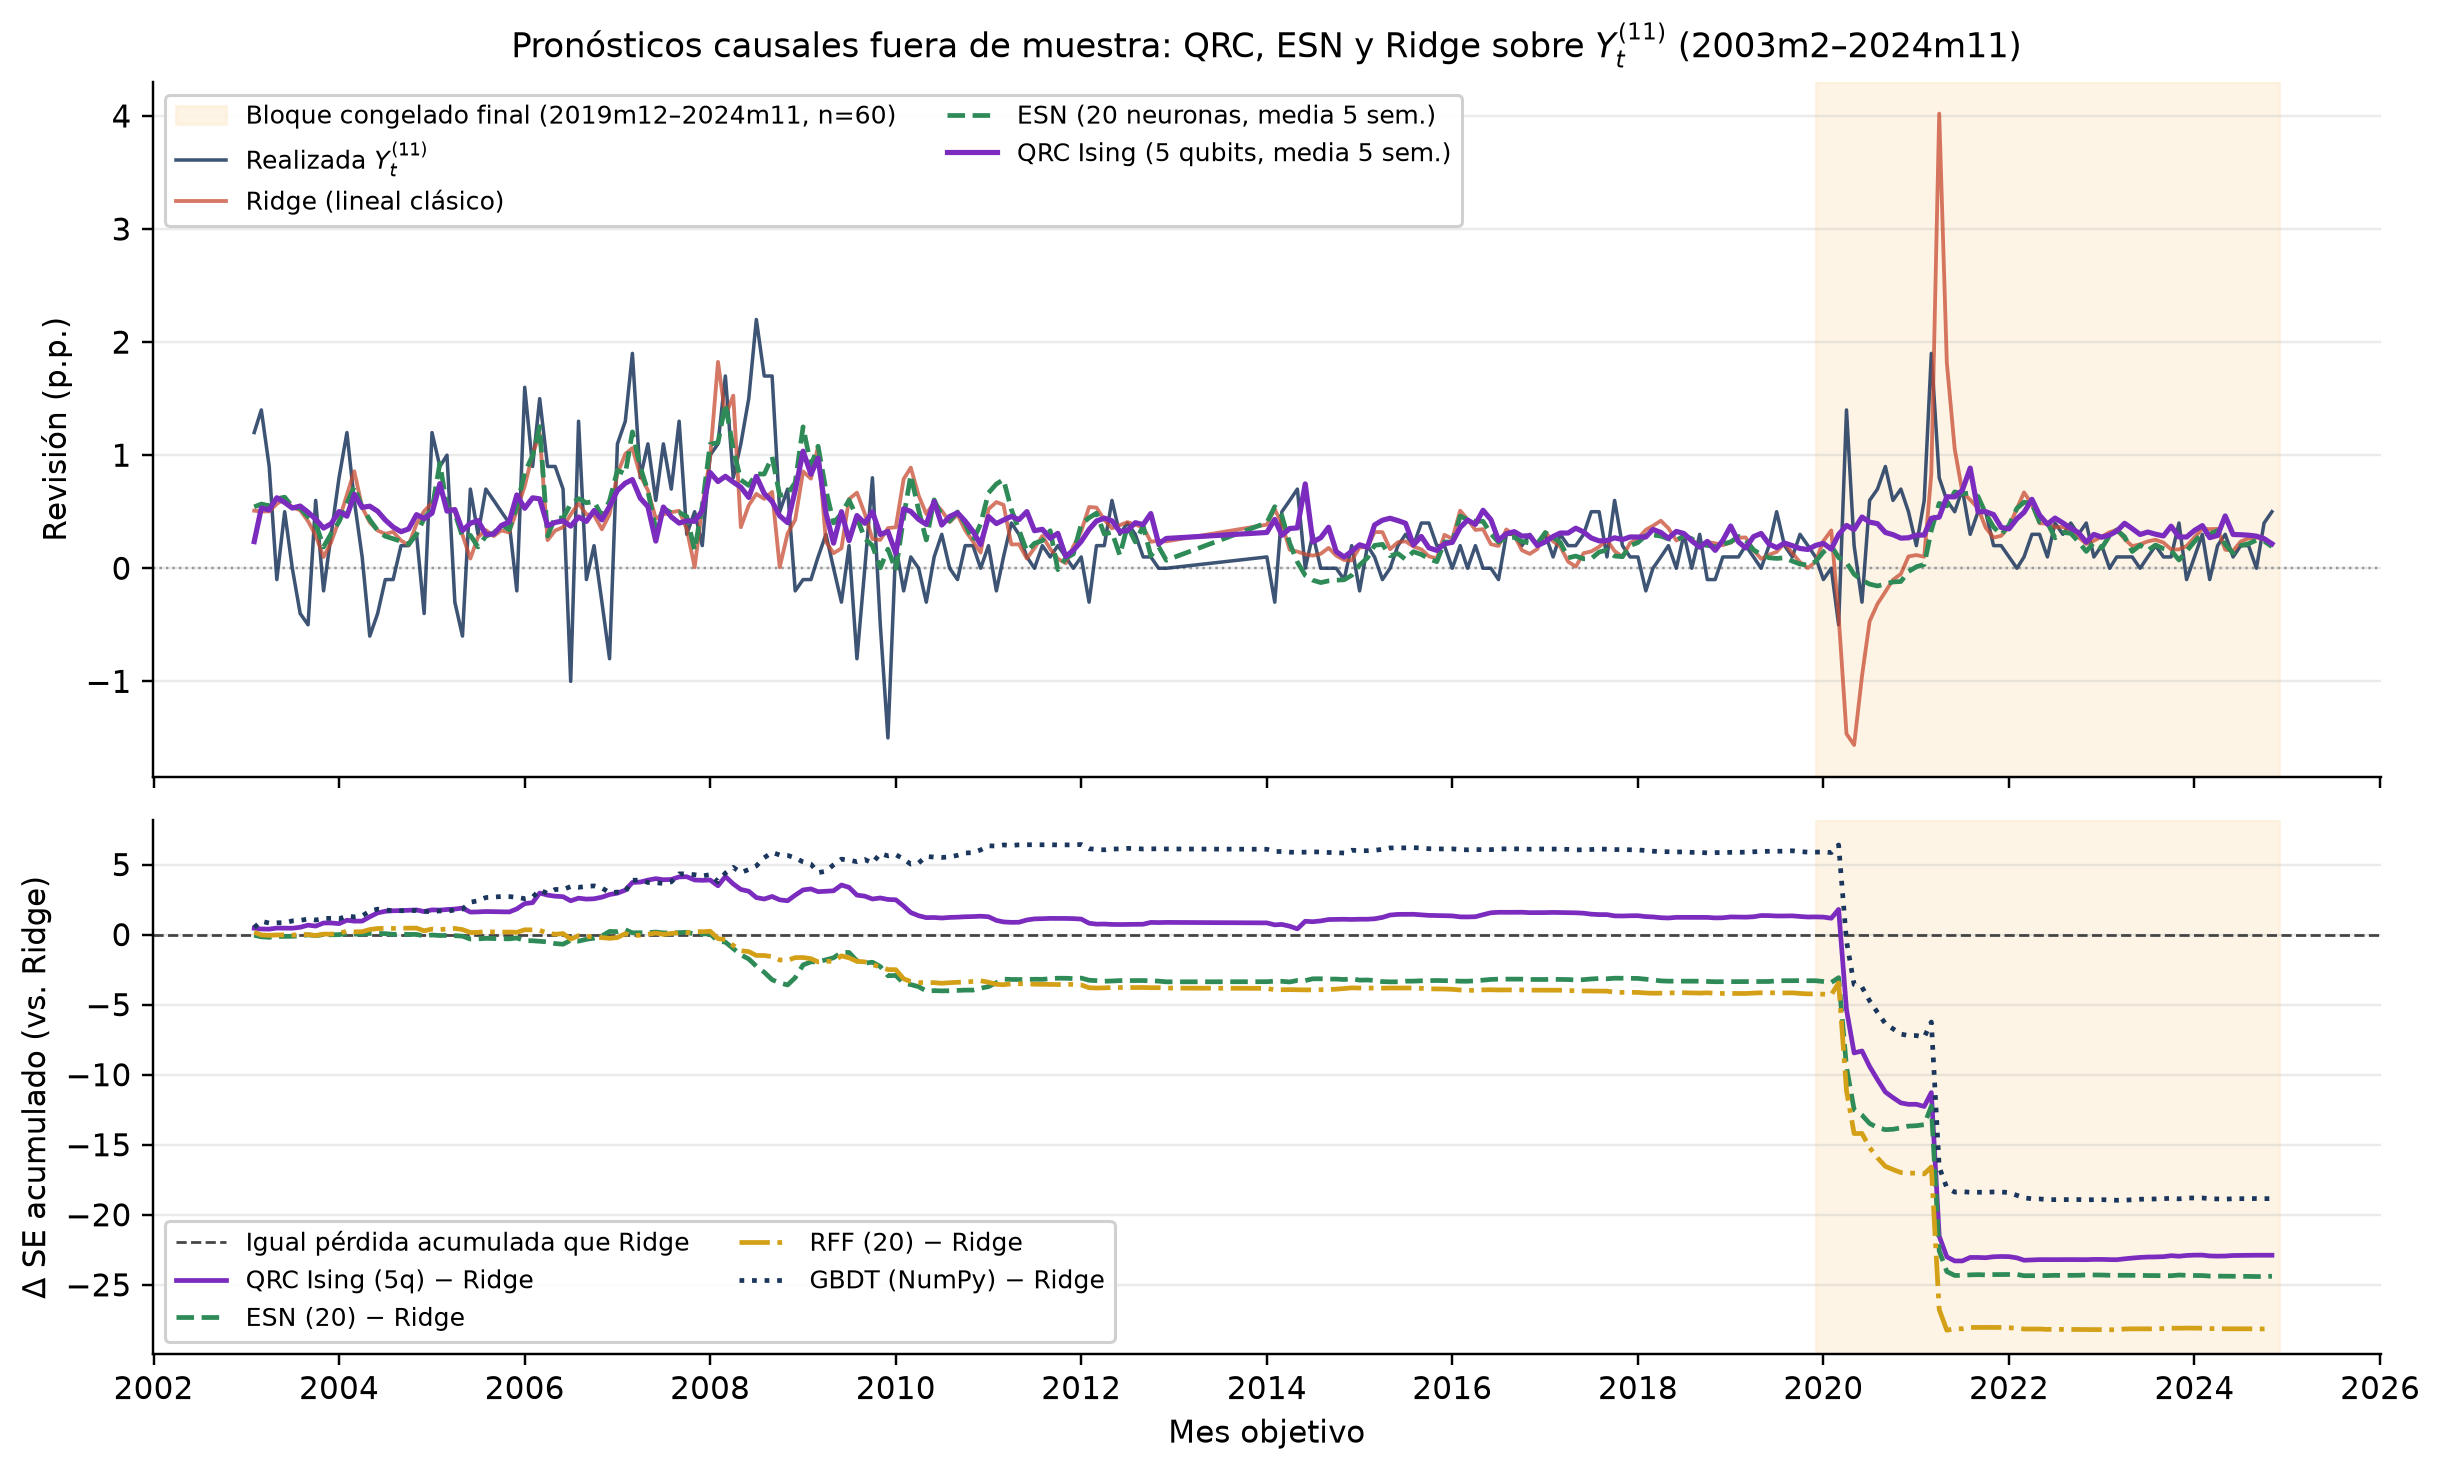
\includegraphics[width=0.96\textwidth]{images/etapa4_reservorios_oos.png}
	\caption{Pronósticos en tiempo real (arriba) y pérdida acumulada frente a Ridge (abajo) para QRC, ESN, RFF y GBDT (2003m2--2024m11).}
	\label{fig:etapa4_oos}
\end{figure}

\begin{figure}[htbp]
	\centering
	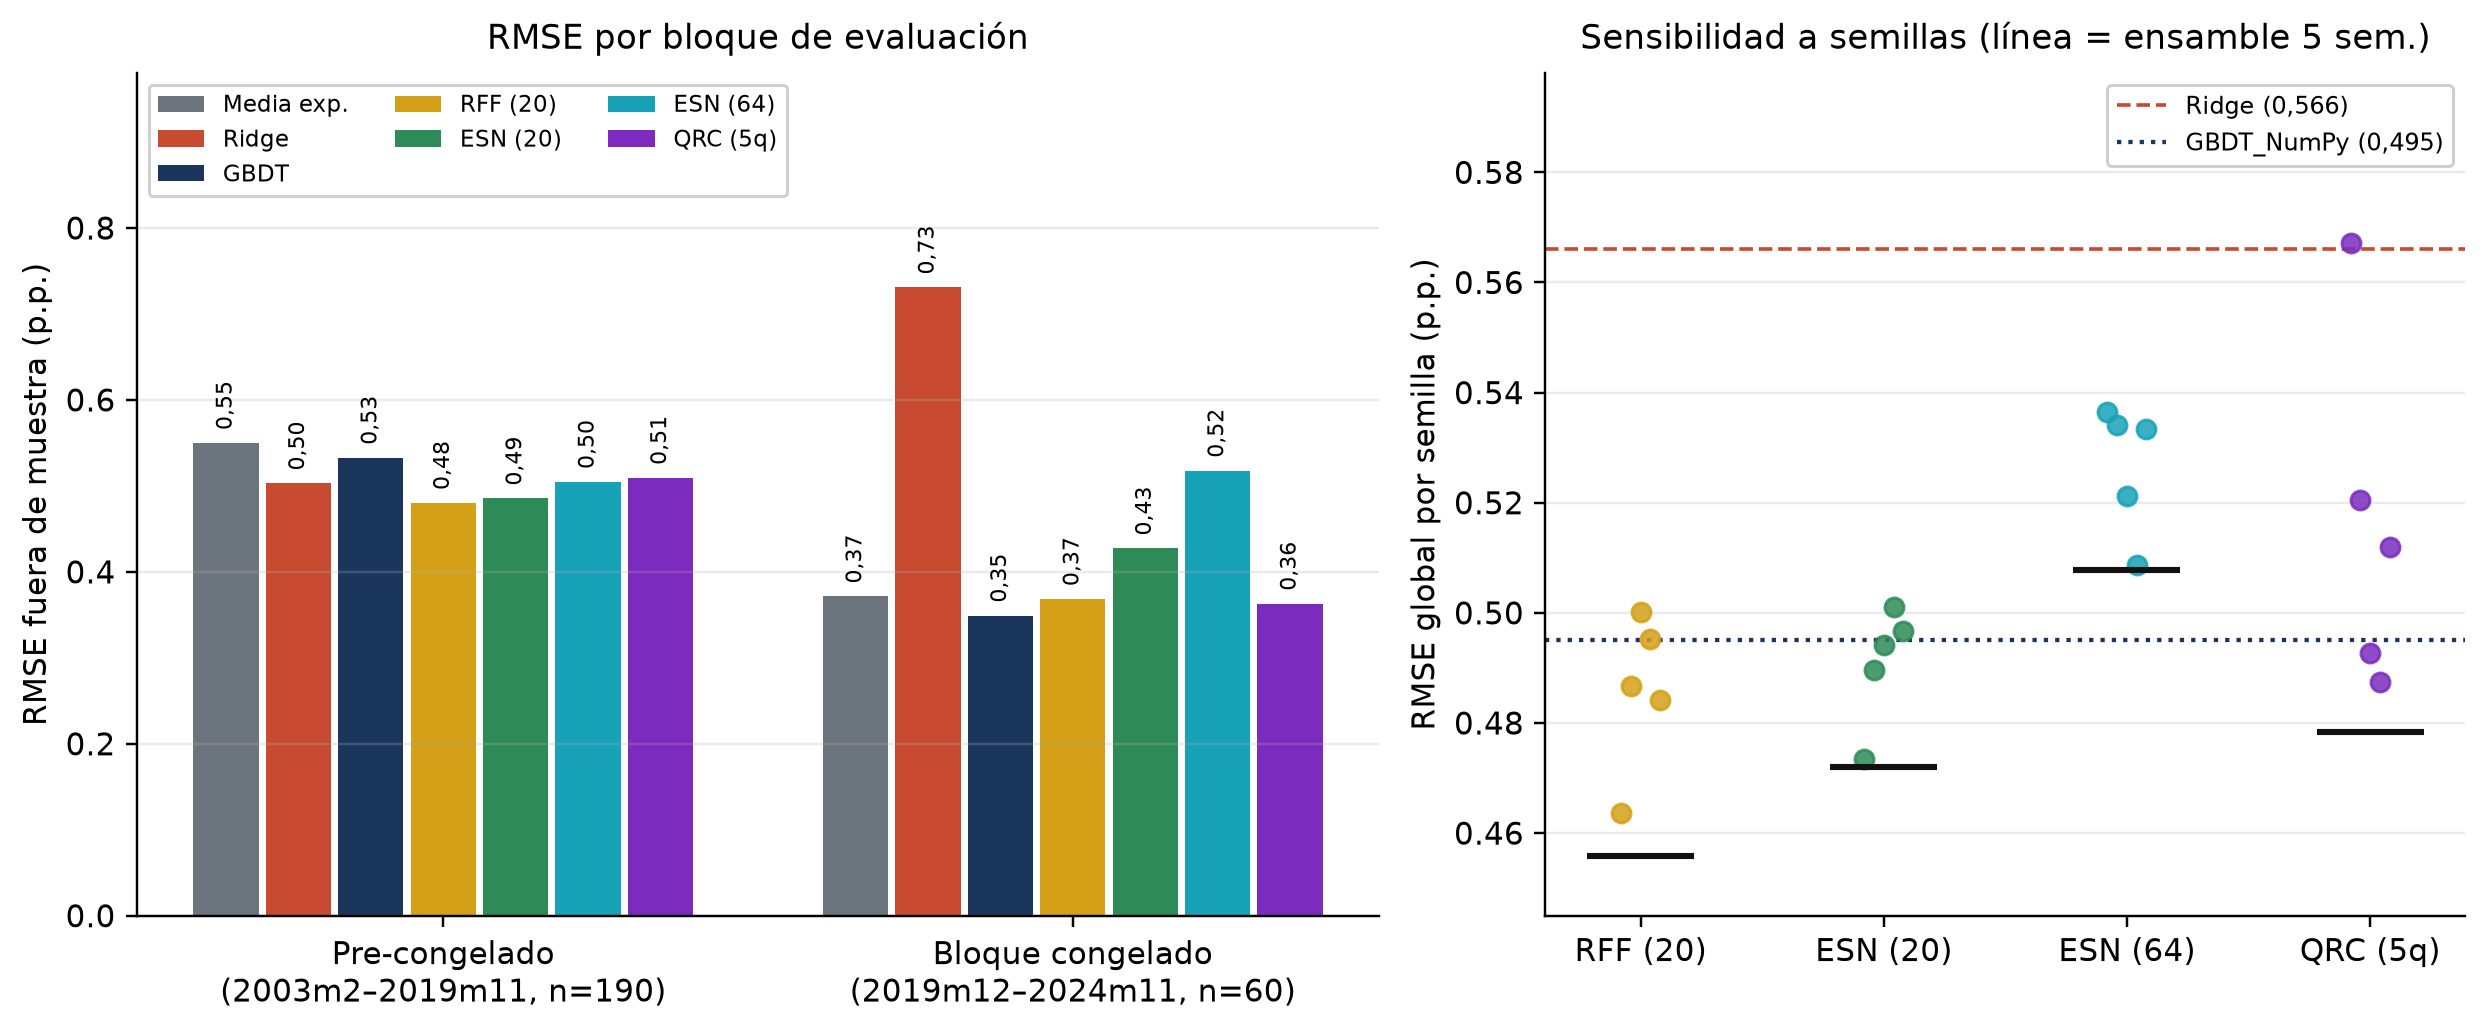
\includegraphics[width=0.96\textwidth]{images/etapa4_estabilidad_regimenes.png}
	\caption{Comparación de RMSE entre período pre-pandemia y tramo final (izquierda) y dispersión entre cinco semillas frente al promedio (derecha).}
	\label{fig:etapa4_estabilidad}
\end{figure}

\subsection{Qué muestran las simulaciones calibradas y cuánta ventaja es detectable}
\label{subsec:experimento_sintetico}

Como una serie histórica única de \(250\) meses puede ocultar situaciones favorables o desfavorables, se construyeron doce escenarios simulados inspirados en los parámetros reales del PBI peruano (\(300\) remuestreos de incertidumbre por bloques sobre \(n=314\) observaciones; Tabla~\ref{tab:etapa6_sintetico} y Figura~\ref{fig:etapa6_delta}). En cada escenario se ejecutaron veinte simulaciones midiendo la mejora porcentual de QRC respecto a cada competidor \(B\):
\[
\Delta_B(\theta)=
100\left(
\frac{\RMSE_{B}(\theta)-\RMSE_{\QRC}(\theta)}
{\RMSE_{B}(\theta)}
\right),
\]
considerando favorable un escenario (\(\theta \in \mathcal{A}\)) solo cuando la mejora superaba el \(2{,}0\%\) mínimo y su intervalo de confianza era positivo.

\begin{table}[htbp]
	\centering
	\caption{Simulaciones calibradas: error RMSE promedio, mejora relativa \(\Delta(\theta)\) de QRC y escenarios favorables (\(\delta_{\min}=2{,}0\%\))}
	\label{tab:etapa6_sintetico}
	\footnotesize
	\renewcommand{\arraystretch}{1.12}
	\begin{tabular}{@{}>{\raggedright\arraybackslash}p{3.9cm}S[table-format=1.3]S[table-format=1.3]S[table-format=1.3]S[table-format=1.3]S[table-format=-2.2]S[table-format=-2.2]c@{}}
		\toprule
		Escenario & {Ridge} & {RFF} & {ESN} & {QRC} & {\(\Delta_{\text{Ridge}}\) (\%)} & {\(\Delta_{\text{ESN}}\) (\%)} & {Favorable?}\\
		\midrule
		Calibrado Perú (\(T=350\)) & 0.606 & 0.617 & 0.620 & 0.652 & -7.49 & -5.08 & No\\
		Muestra mediana (\(T=700\)) & 0.619 & 0.629 & 0.638 & 0.669 & -8.53 & -5.29 & No\\
		Muestra larga (\(T=1400\)) & 0.642 & 0.649 & 0.662 & 0.695 & -8.42 & -5.06 & No\\
		Persistencia baja (\(\phi=0{,}10\)) & 0.640 & 0.642 & 0.645 & 0.647 & -1.32 & -0.45 & No\\
		Persistencia alta (\(\phi=0{,}65\)) & 0.664 & 0.701 & 0.724 & 0.801 & -20.90 & -11.16 & No\\
		Señal baja (\(0{,}5\times\)) & 0.655 & 0.665 & 0.669 & 0.680 & -3.62 & -1.32 & No\\
		Señal alta (\(2{,}5\times\)) & 0.638 & 0.652 & 0.665 & 0.705 & -11.62 & -6.67 & No\\
		Ruido normal sin cambios (\(T=350\)) & 0.630 & 0.646 & 0.649 & 0.672 & -6.39 & -3.45 & No\\
		No lineal + choques (\(T=350\)) & 0.615 & 0.621 & 0.620 & 0.634 & -2.99 & -2.13 & No\\
		No lineal + choques (\(T=1000\)) & 0.624 & 0.618 & 0.617 & 0.633 & -1.36 & -2.41 & No\\
		Pocas variables (\(d=2\)) & 0.622 & 0.631 & 0.631 & 0.656 & -5.87 & -4.05 & No\\
		Muchas variables (\(d=8\)) & 0.693 & 0.715 & 0.723 & 0.753 & -8.48 & -4.14 & No\\
		\bottomrule
	\end{tabular}
	\fuente{elaboración propia con base en las simulaciones calibradas del estudio (\(20\) repeticiones por escenario).}
\end{table}

Las conclusiones de los doce mundos simulados son consistentes:
\begin{enumerate}
	\item \textbf{Ningún escenario favoreció al modelo cuántico (\(\mathcal{A}=\emptyset\)):} QRC no ganó en ninguno de los doce casos probados, ni siquiera al aumentar el historial a \(1\,400\) meses (donde siguió \(8{,}4\%\) por detrás de Ridge). Esto confirma que en el Perú no venció a Ridge por mérito cuántico, sino porque la pandemia hizo fallar las rectas lineales y por promediar cinco semillas.
	\item \textbf{Donde hay memoria lineal fuerte, QRC pierde más:} cuando el patrón anual es intenso (\(\phi=0{,}65\)), transformar las variables en ángulos cuánticos distorsiona esa relación simple y QRC queda \(20{,}90\%\) por detrás de Ridge.
	\item \textbf{Con curvas y choques fuertes también ganan los modelos clásicos:} cuando la economía artificial incluye choques bruscos y \(1\,000\) meses, ESN (\(0{,}617\)) y RFF (\(0{,}618\)) superan a Ridge (\(0{,}624\)) y mantienen cerca de \(2{,}3\%\) de ventaja sobre QRC (\(0{,}633\)).
\end{enumerate}

Además, se calculó cuánta ventaja real haría falta en los \(250\) meses peruanos para que las pruebas estadísticas la detecten con seguridad al \(80\%\) (Figura~\ref{fig:etapa6_potencia} y Anexo~\ref{app:potencia}). Debido a la fuerte agitación de la pandemia, frente a Ridge se necesitaría una mejora enorme de \(36{,}1\%\) para probar ventaja con certeza; y frente a los controles clásicos más estables se necesitaría entre \(5{,}7\%\) (RFF), \(7{,}6\%\) (media histórica) y \(11{,}1\%\) (ESN). En otras palabras, con el tamaño actual de la serie peruana no es posible distinguir con seguridad mejoras pequeñas del orden del \(2\%\).

\begin{figure}[htbp]
	\centering
	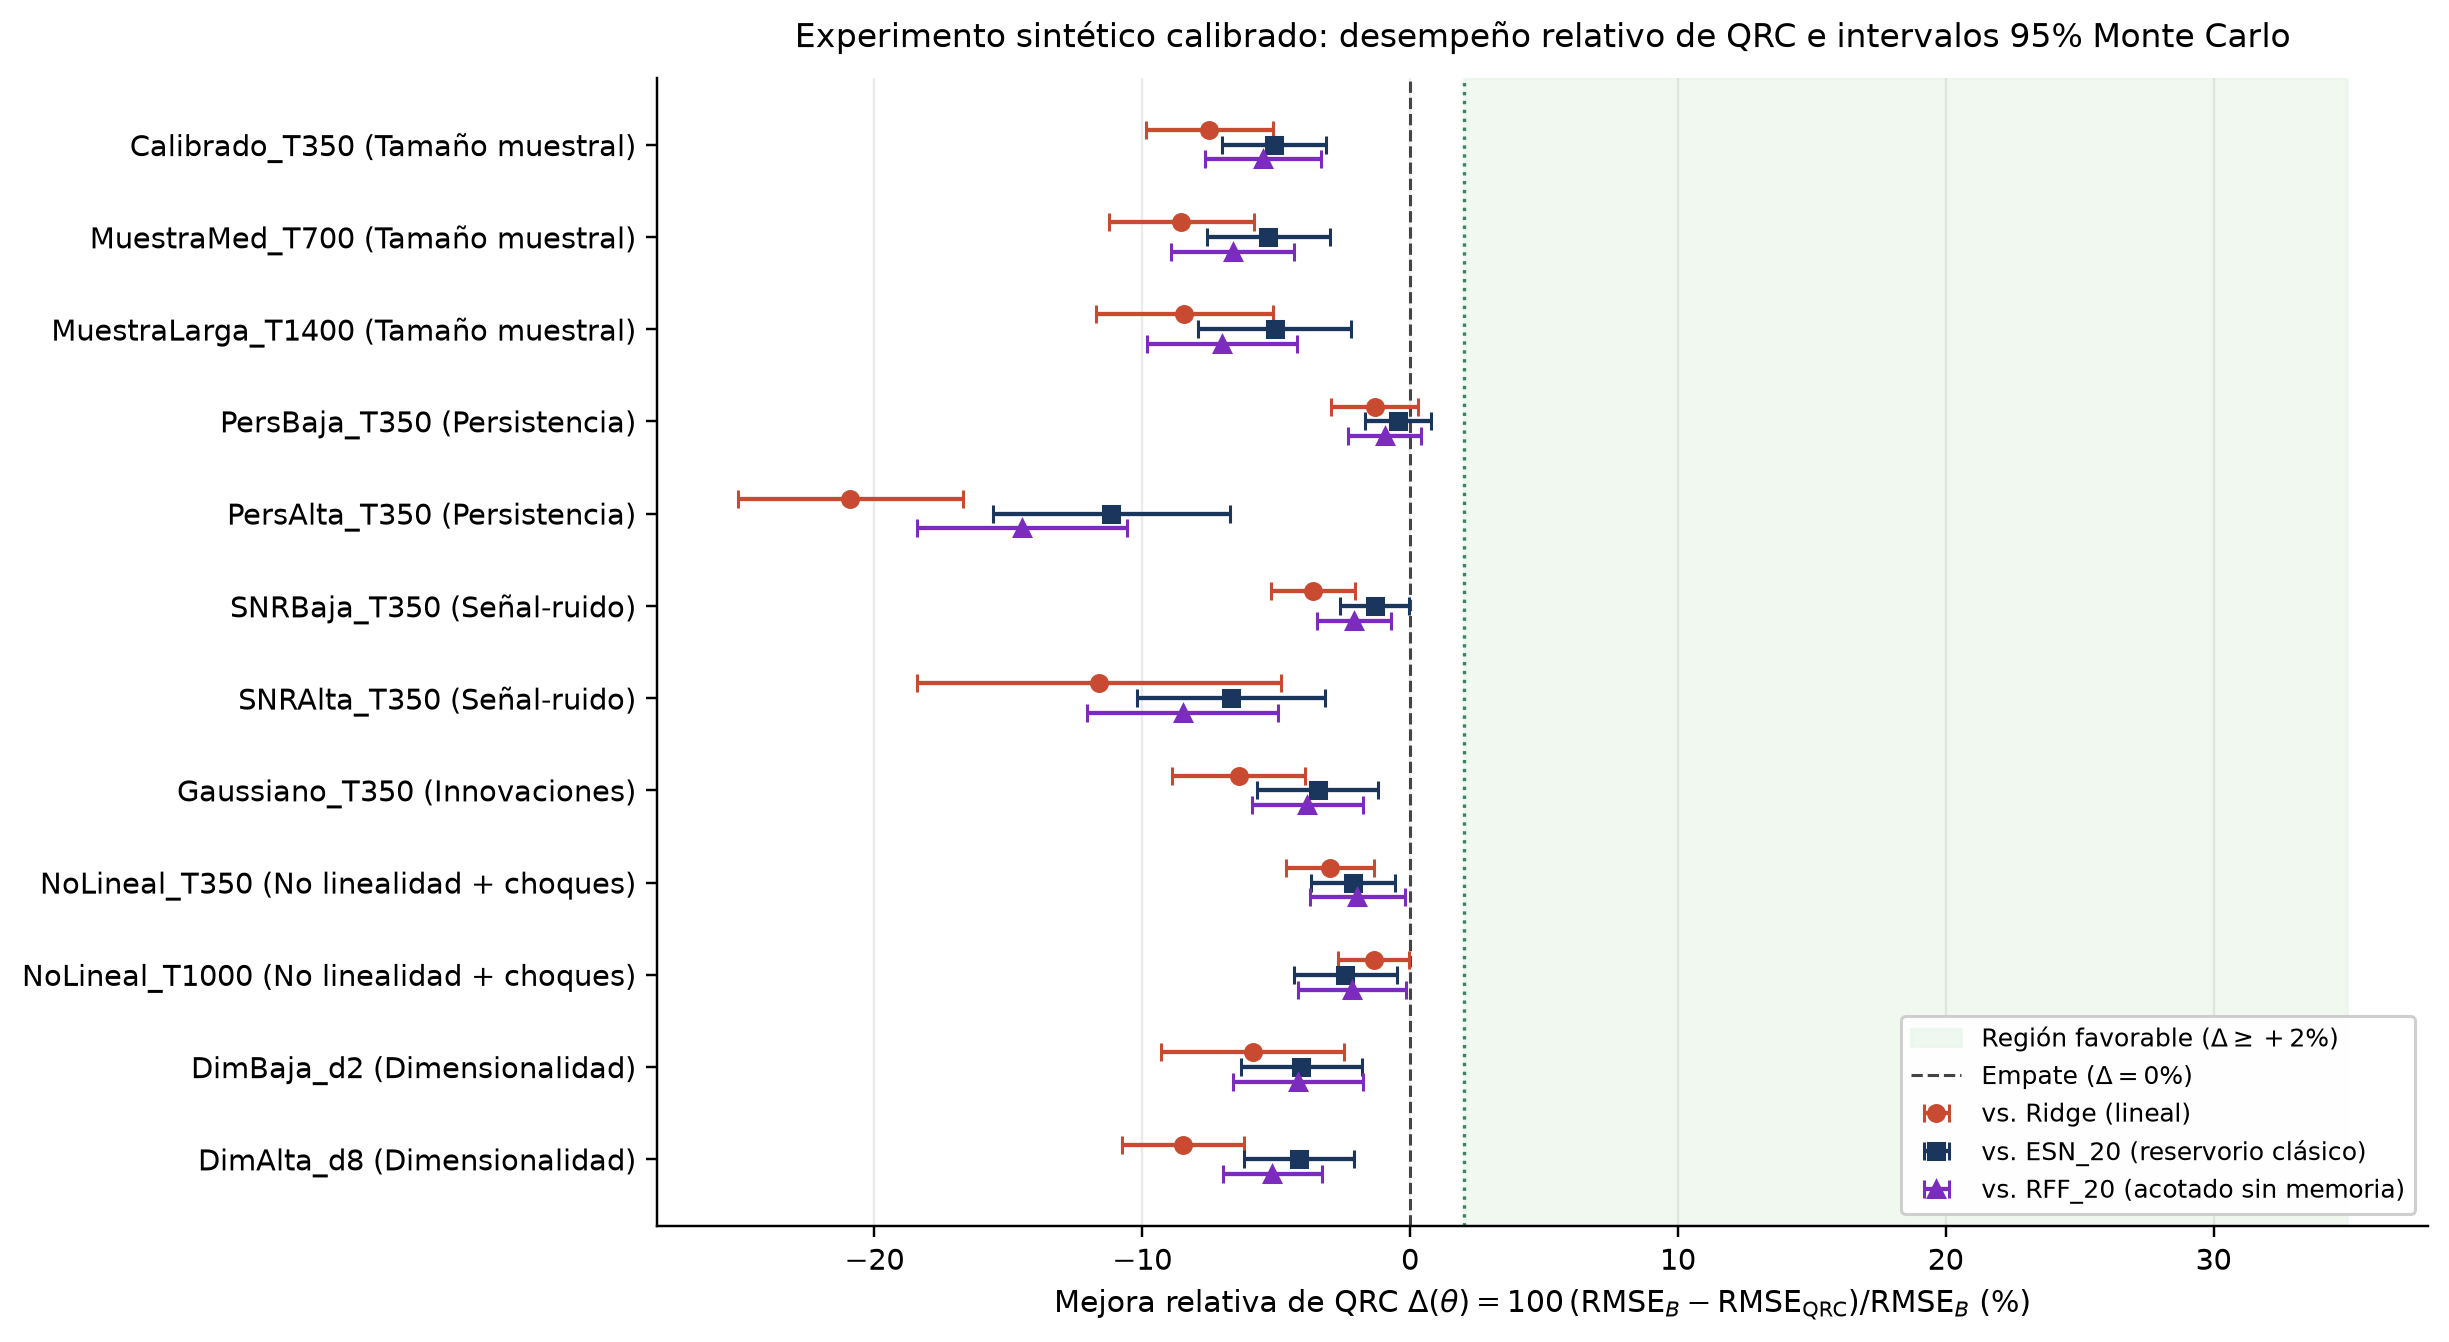
\includegraphics[width=0.96\textwidth]{images/etapa6_delta_escenarios.png}
	\caption{Diferencia porcentual relativa \(\Delta(\theta)\) de QRC e intervalos al 95\% en los doce escenarios simulados.}
	\label{fig:etapa6_delta}
\end{figure}

\begin{figure}[htbp]
	\centering
	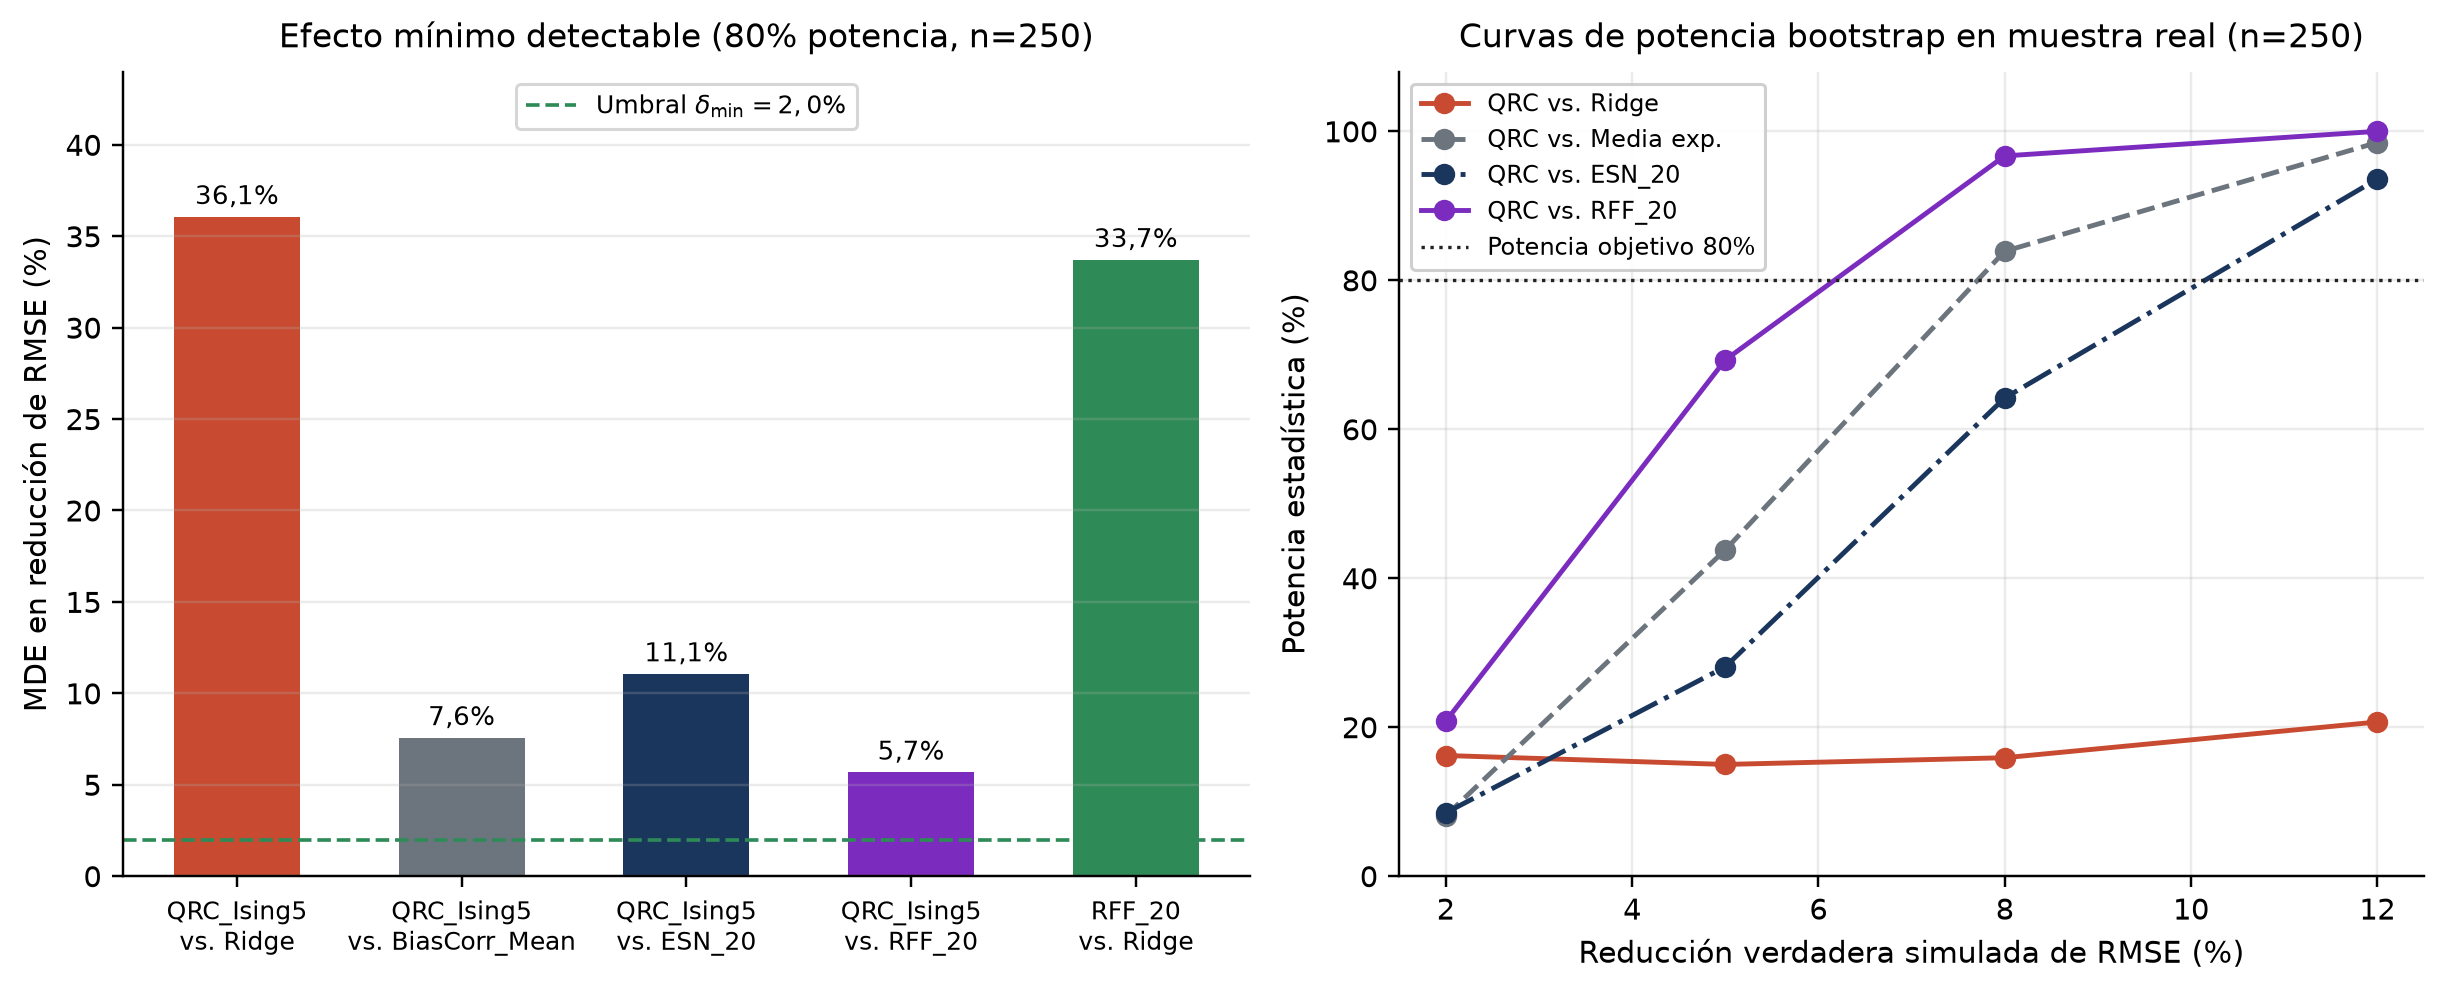
\includegraphics[width=0.96\textwidth]{images/etapa6_potencia_mde.png}
	\caption{Mejora mínima detectable con 80\% de seguridad (izquierda) y probabilidad de detección según tamaño real de ganancia en \(n=250\) orígenes (derecha).}
	\label{fig:etapa6_potencia}
\end{figure}

\subsection{Por qué no se realizó la evaluación económica}
\label{subsec:analisis_economico}

De acuerdo con la regla fijada desde el inicio (Anexo~\ref{app:voi}), solo se estimarían ganancias o pérdidas monetarias si QRC superaba de forma clara y robusta tanto a Ridge como a sus pares clásicos. Al no ganar ninguna comparación múltiple, quedar por detrás de RFF y no mostrar ventaja en las simulaciones (\(\mathcal{A}=\emptyset\)), la evaluación económica se detuvo para no atribuir beneficios económicos artificiales.

\subsection{Pruebas conjuntas finales para evitar falsos positivos}
\label{subsec:inferencia_integrada_etapa8}

Cuando se comparan varios modelos a la vez, algún resultado puede parecer significativo simplemente por suerte. Para evitarlo, la Tabla~\ref{tab:etapa8_holm} aplica correcciones por comparaciones múltiples \parencite{holm1979,benjamini1995} sobre los siete contrastes principales de QRC, y la Tabla~\ref{tab:etapa8_mcs} (junto con la Figura~\ref{fig:etapa8_mcs}) aplica el método del conjunto de confianza de modelos de \textcite{hansen2011}, que agrupa a todos los modelos que estadísticamente siguen empatados en precisión.

\begin{table}[htbp]
	\centering
	\caption{Comparaciones directas de QRC con ajuste por pruebas múltiples}
	\label{tab:etapa8_holm}
	\scriptsize
	\setlength{\tabcolsep}{3.5pt}
	\renewcommand{\arraystretch}{1.14}
	\begin{tabular}{@{}>{\raggedright\arraybackslash}p{3.1cm}S[table-format=1.3]S[table-format=-1.3]cS[table-format=1.4]S[table-format=1.4]S[table-format=1.4]>{\raggedright\arraybackslash}p{2.7cm}@{}}
		\toprule
		Comparador (\(n=250\)) & {\(\text{RMSE}\)} & {\(\Delta\)} & {\(\text{IC}_{95\%}\) boot.} & {\(p_{\text{DM}}\)} & {\(p_{\text{Holm}}\)} & {\(p_{\text{BH}}\)} & Resultado formal\\
		\midrule
		Referencia nula (\(\widehat{Y}=0\)) & 0.574 & -0.096 & \([-0{,}191;\, 0{,}002]\) & 0.1131 & 0.5656 & 0.2640 & Resultado inconcluso\\
		Corrección media exp. & 0.513 & -0.034 & \([-0{,}060;\, -0{,}010]\) & 0.0175 & 0.1052 & 0.0614 & Mejora sin sig. Holm\\
		Autorregresivo AR (BIC) & 0.498 & -0.020 & \([-0{,}057;\, 0{,}019]\) & 0.3811 & 0.8094 & 0.4447 & Resultado inconcluso\\
		Regresión Ridge & 0.566 & -0.088 & \([-0{,}208;\, 0{,}020]\) & 0.1957 & 0.7830 & 0.3426 & Resultado inconcluso\\
		Árboles potenciados (GBDT) & 0.495 & -0.017 & \([-0{,}044;\, 0{,}008]\) & 0.2698 & 0.8094 & 0.3777 & Resultado inconcluso\\
		ESN clásica (20 neuronas) & 0.472 & 0.006 & \([-0{,}032;\, 0{,}038]\) & 0.7296 & 0.8094 & 0.7296 & Resultado inconcluso\\
		Características aleatorias (RFF) & 0.456 & 0.022 & \([+0{,}006;\, +0{,}038]\) & 0.0146 & 0.1023 & 0.0614 & Desventaja sin sig. Holm\\
		\midrule
		\multicolumn{8}{@{}l}{\textit{Único contraste significativo tras Holm en los subperíodos (pre-pandemia \(n=190\)):}}\\
		Características RFF (pre-COVID) & 0.480 & 0.029 & \([+0{,}012;\, +0{,}046]\) & 0.0038 & 0.0265 & 0.0265 & Evidencia desfavorable\\
		\bottomrule
	\end{tabular}
	\fuente{elaboración propia a partir de las pruebas comparativas del estudio. \(\text{RMSE}_{\text{QRC}}=0{,}478\) en \(n=250\) y \(0{,}509\) en \(n=190\); \(\Delta=\text{RMSE}_{\text{QRC}}-\text{RMSE}_{\text{comp}}<0\) favorece a QRC.}
\end{table}

La Tabla~\ref{tab:etapa8_holm} deja dos certezas simples: primero, la pequeña ventaja puntual de QRC sobre el promedio histórico (\(p=0{,}0175\) aislado) pierde validez al corregir por comparaciones múltiples (\(p_{\text{Holm}}=0{,}1052\)); segundo, el único contraste firme tras corrección ocurre \textbf{en contra de QRC}, pues antes de la pandemia el método clásico RFF logra mayor precisión estadística (\(p_{\text{Holm}}=0{,}0265\)). En el bloque final de \(60\) meses todos los contrastes ajustados marcan empate estadístico (\(p_{\text{Holm}}=1{,}000\)).

\begin{table}[htbp]
	\centering
	\caption{Permanencia de los doce modelos dentro del grupo de mejores modelos empatados (\(p_{\text{MCS}}\))}
	\label{tab:etapa8_mcs}
	\footnotesize
	\setlength{\tabcolsep}{5.5pt}
	\renewcommand{\arraystretch}{1.12}
	\begin{tabular}{@{}>{\raggedright\arraybackslash}p{4.4cm}S[table-format=1.3]S[table-format=1.3]S[table-format=1.3]S[table-format=1.3]S[table-format=1.3]S[table-format=1.3]@{}}
		\toprule
		& \multicolumn{2}{c}{Global (\(n=250\))} & \multicolumn{2}{c}{Pre-pandemia (\(n=190\))} & \multicolumn{2}{c}{Tramo final (\(n=60\))}\\
		\cmidrule(lr){2-3} \cmidrule(lr){4-5} \cmidrule(lr){6-7}
		Modelo & {MSE} & {MAE} & {MSE} & {MAE} & {MSE} & {MAE}\\
		\midrule
		Características aleatorias (RFF) & 1.000 & 1.000 & 1.000 & 1.000 & 0.713 & 0.880\\
		Reservorio clásico ESN (20 n.) & 0.674 & 0.827 & 0.767 & 0.922 & 0.584 & 0.880\\
		Reservorio cuántico QRC (5 qubits) & 0.674 & 0.827 & 0.767 & 0.922 & 0.713 & 0.880\\
		Árboles potenciados (GBDT) & 0.674 & 0.827 & 0.549 & 0.708 & 1.000 & 1.000\\
		Autorregresivo AR (BIC) & 0.674 & 0.827 & 0.767 & 0.922 & 0.584 & 0.880\\
		Reservorio clásico ESN (64 n.) & 0.674 & 0.827 & 0.767 & 0.922 & 0.378 & 0.442\\
		Corrección de sesgo (media exp.) & 0.640 & 0.512 & 0.097 & 0.003 & 0.713 & 0.880\\
		Corrección de sesgo (móvil 60m) & 0.640 & 0.827 & 0.118 & 0.247 & 0.713 & 0.880\\
		ARX observable (BIC) & 0.640 & 0.827 & 0.549 & 0.922 & 0.346 & 0.442\\
		Regresión Ridge (benchmark) & 0.640 & 0.827 & 0.767 & 0.922 & 0.187 & 0.243\\
		Referencia nula (\(\widehat{Y}=0\)) & 0.640 & 0.827 & 0.549 & 0.922 & 0.353 & 0.442\\
		Factores dinámicos (DFM + Ridge) & 0.562 & 0.736 & 0.767 & 0.922 & 0.222 & 0.201\\
		\bottomrule
	\end{tabular}
	\fuente{elaboración propia a partir de la evaluación conjunta del estudio (\(T_{\max}\), \(B=2000\)). Se mantiene en el grupo ganador al 90\% si \(p_{\text{MCS}}\ge 0{,}10\) (y al 75\% si \(p_{\text{MCS}}\ge 0{,}25\)).}
\end{table}

El análisis conjunto de la Tabla~\ref{tab:etapa8_mcs} y la Figura~\ref{fig:etapa8_mcs} resume toda la evaluación:
\begin{itemize}
	\item \textbf{En toda la muestra (2003--2024):} ninguno de los doce modelos queda descartado definitivamente, aunque RFF ocupa el primer lugar (\(p_{\text{MCS}}=1{,}000\)) y ESN, QRC, AR y GBDT forman un grupo equivalente detrás.
	\item \textbf{Separando épocas normales y pandemia:} antes de 2020, el método descarta la simple corrección por promedio histórico (\(p=0{,}097\)); mientras que durante la pandemia, encabezan los árboles potenciados (\(p=1{,}000\)), seguidos de RFF y QRC (\(p=0{,}713\)), expulsando del grupo líder al 75\% a los modelos lineales no acotados (Ridge, \(p=0{,}187\); factores dinámicos, \(p=0{,}222\)).
\end{itemize}

\begin{figure}[htbp]
	\centering
	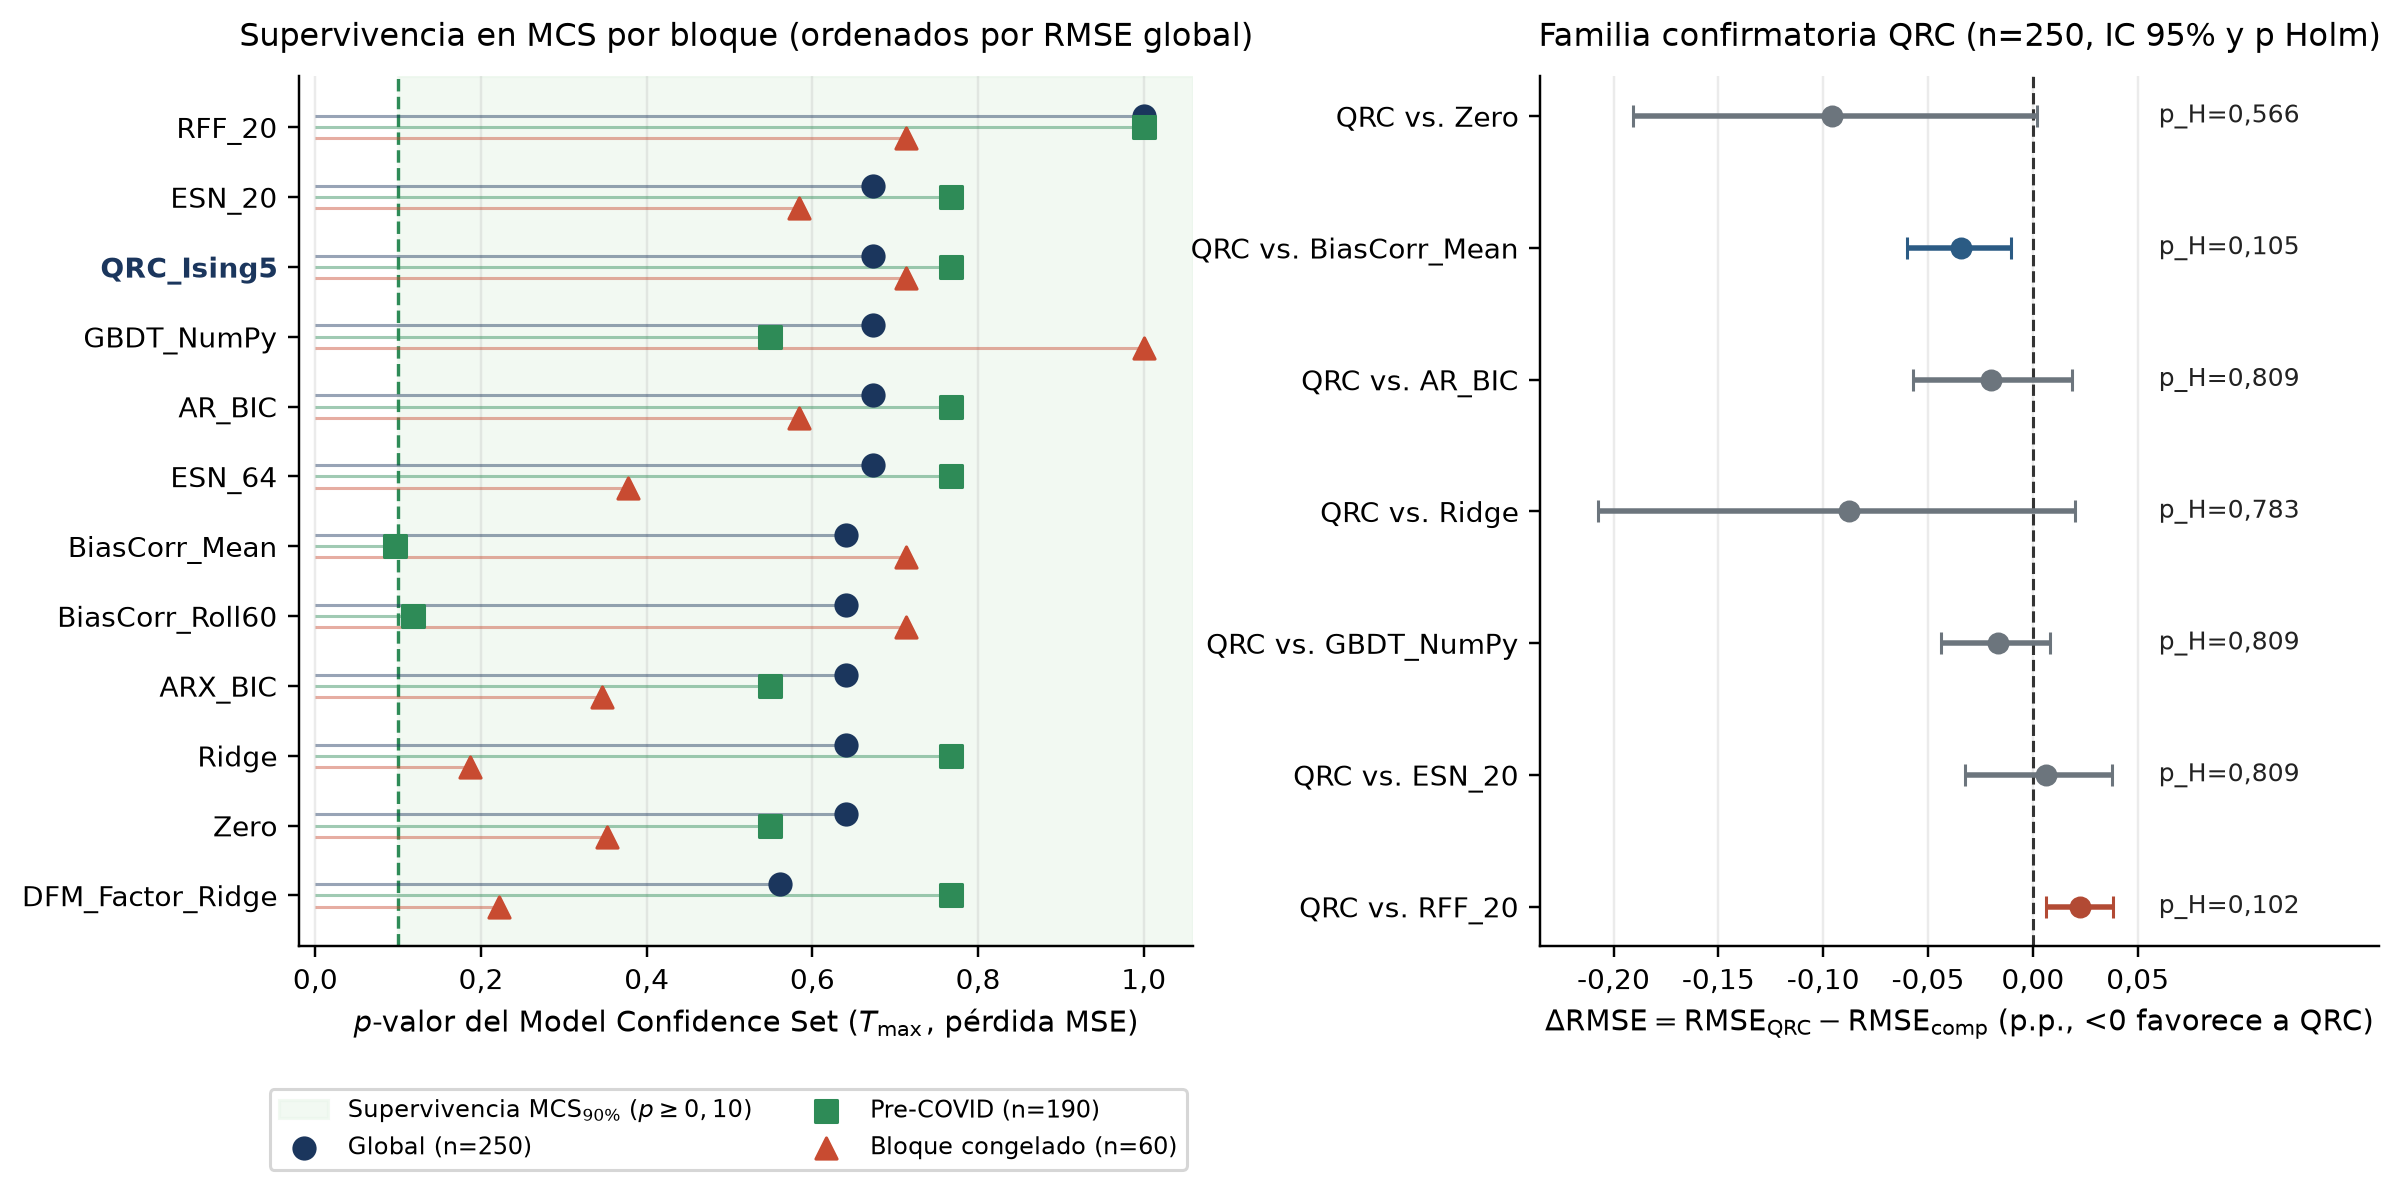
\includegraphics[width=0.98\textwidth]{images/etapa8_mcs_inferencia.png}
	\caption{Supervivencia en el grupo de mejores modelos por época (izquierda) y comparaciones directas de QRC en \(n=250\) con márgenes al 95\% (derecha).}
	\label{fig:etapa8_mcs}
\end{figure}

	% ============================================================================
\section{Discusión}

Los hallazgos obtenidos permiten responder con claridad a las cuatro interrogantes que guiaron la investigación y contrastarlos con la literatura sobre datos macroeconómicos en tiempo real.

En primer lugar, respecto del carácter sistemático de las revisiones, los resultados confirman lo planteado por \textcite{croushore2011} y el análisis entre nueva información y ruido de medición \parencite{mankiw1986}: a horizonte continuo de once meses (\(n=350\)), las primeras publicaciones del PBI peruano no actúan como pronósticos racionales insesgados. Muestran una subestimación promedio positiva y robusta de \(+0{,}347\) puntos porcentuales (\(p=5{,}3\times 10^{-8}\)), persistencia anual detectable en tiempo real (\(\hat{\rho}_{12}=+0{,}386\)), colas pesadas y rechazo de eficiencia de \textcite{mincer1969} debido al intercepto positivo constante, patrón que persiste incluso después de retirar los cruces de cambio de año base de 2000 y 2014.

En segundo lugar, en cuanto al desempeño de los referentes clásicos, los modelos muestran un comportamiento claramente distinto antes y después de la pandemia. En el tramo previo a 2020 (\(n=190\)), la regresión Ridge aprovecha de manera eficaz las señales sectoriales y los rezagos anuales observables (\(\text{RMSE}=0{,}503\), \(R^2_{\text{OOS}}=+0{,}094\)), superando con significancia estadística a la corrección por media histórica (\(p=0{,}0071\)). Sin embargo, al incluir las variaciones extremas de 2020 y 2021 (\(-40{,}5\)\% y \(+58{,}5\)\%), los modelos lineales sin acotamiento extrapolan fuera de rango y elevan fuertemente su error en el bloque final (\(\text{RMSE}=0{,}731\)). En cambio, las técnicas clásicas acotadas evitan ese colapso: las características aleatorias de Fourier (RFF) alcanzan la mayor precisión global (\(\text{RMSE}=0{,}456\), \(R^2_{\text{OOS}}=+0{,}149\)) y los árboles potenciados acotados (GBDT) obtienen el menor error en el tramo pandémico (\(\text{RMSE}=0{,}349\), \(R^2_{\text{OOS}}=+0{,}087\)).

En tercer lugar, al evaluar el aporte específico del reservorio cuántico (QRC), los resultados muestran que su ventaja frente a la predicción nula o la corrección media clásica (\(\text{RMSE}=0{,}478\) global y \(0{,}363\) en el bloque final; \(p=0{,}0175\) sin ajuste frente a la media histórica) se explica por el acotamiento natural de sus variables de salida, mas no por superioridad cuántica intrínseca. Frente a referentes clásicos no lineales de igual dimensión de lectura, QRC empata estadísticamente con la red clásica de estado eco ESN (\(p=0{,}730\)), queda por debajo de RFF (\(p=0{,}0146\) global sin ajuste y \(p_{\text{Holm}}=0{,}0265\) antes de la pandemia) y presenta mayor variabilidad entre semillas aleatorias. Tal como preveía el diseño, este resultado negativo controlado constituye evidencia empírica valiosa para evitar atribuir ventajas injustificadas a modelos cuánticos en series macroeconómicas cortas.

En cuarto lugar, el experimento sintético calibrado y el análisis de potencia ayudan a entender por qué no surge una ventaja cuántica clara. La simulación sobre doce escenarios revela una región favorable vacía (\(\mathcal{A}=\emptyset\)) incluso al ampliar la muestra hasta \(1\,400\) períodos, debido a que la codificación angular no lineal distorsiona la señal cuando la persistencia lineal \(\phi_{12}\) es alta (\(-20{,}90\)\% frente a Ridge). Además, el análisis de potencia sobre las diferencias observadas en la muestra peruana (\(n=250\)) indica que se requerirían reducciones de error de entre \(5{,}7\)\% y \(11{,}1\)\% frente a controles clásicos acotados (\(36{,}1\)\% frente a Ridge) para lograr una potencia del 80\%, lo cual explica la amplitud del conjunto de confianza de modelos global y muestra que las series disponibles no permiten discriminar ganancias pequeñas del 2\%.

Por último, el análisis de sensibilidad confirmó la estabilidad cualitativa del sesgo positivo entre \(H=11\) y los horizontes alternativos (\(H=12, 6, 3\)) y mostró que la no linealidad detectada en la prueba RESET proviene del episodio pandémico. Cabe delimitar tres restricciones objetivas del estudio: primero, la base trabaja en régimen mensual aproximado al tiempo real ante la falta de fecha calendario diaria y el inicio posterior de los sectores de electricidad y servicios; segundo, los modelos de árboles y el circuito de cinco qubits se ejecutaron mediante simulaciones matemáticas exactas en Python sin ruido de hardware físico; y tercero, al no verificarse superioridad predictiva estable sobre los controles clásicos, se mantuvo detenida la evaluación económica condicionada sin generar beneficios monetarios hipotéticos.

	% ============================================================================
\section{Conclusiones}

Completado todo el análisis empírico, de simulación y de inferencia estadística planteado en el estudio, se formulan las conclusiones finales de acuerdo con el objetivo general y los objetivos específicos:

Respecto del objetivo general, la evaluación fuera de muestra sobre las revisiones del PBI peruano (\(n=250\), 2003--2024) demuestra que la computación de reservorio cuántico de cinco qubits supera puntualmente a la referencia nula y a la corrección clásica por media histórica (\(\text{RMSE}=0{,}478\) frente a \(0{,}513\), \(p=0{,}0175\) sin ajuste), pero \textbf{no mejora a los controles clásicos no lineales comparables} de igual dimensión de lectura: empata estadísticamente con la red clásica de estado eco ESN (\(\text{RMSE}=0{,}472\), \(p=0{,}730\)), es superada por características aleatorias de Fourier (\(\text{RMSE}=0{,}456\), con significancia tras ajustar por Holm--Bonferroni en el período previo a la pandemia, \(p_{\text{Holm}}=0{,}0265\)) y queda por debajo de los árboles potenciados acotados durante el choque pandémico (\(\text{RMSE}=0{,}349\) frente a \(0{,}363\)). En la familia confirmatoria global ningún contraste supera el umbral ajustado por multiplicidad (\(p_{\text{Holm}}\ge 0{,}1023\)), y el conjunto de confianza de modelos retiene conjuntamente a los competidores clásicos junto a QRC.

En relación con los objetivos específicos, se concluye que:
\begin{enumerate}
	\item \textbf{Propiedades estadísticas de las revisiones:} en la muestra depurada sin cambios de año base a horizonte continuo de once meses (\(n=350\)), las revisiones del PBI peruano presentan una estructura sistemática clara (Hipótesis~1), caracterizada por un sesgo positivo robusto de \(+0{,}347\) puntos porcentuales (\(p=5{,}3\times 10^{-8}\)), colas pesadas (curtosis en exceso de \(6{,}293\)), heterocedasticidad condicional, persistencia anual observable en tiempo real (\(\hat{\rho}_{12}=+0{,}386\)) y no linealidad concentrada únicamente en los años de pandemia 2020--2024.
	\item \textbf{Desempeño de referentes clásicos ante choques extremos:} antes de diciembre de 2019 (\(n=190\)), la regresión Ridge encabeza los métodos lineales tradicionales (\(\text{RMSE}=0{,}503\), \(R^2_{\text{OOS}}=+0{,}094\)); sin embargo, ante las caídas y rebotes atípicos de 2020--2021, las especificaciones lineales sin acotamiento extrapolan de forma excesiva (\(\text{RMSE}=0{,}731\) en el tramo final, quedando fuera del conjunto de confianza al \(75\)\%), mientras los métodos acotados (RFF, árboles potenciados y reservorios) evitan dicho deterioro.
	\item \textbf{Condiciones sintéticas y potencia estadística:} en doce escenarios calibrados sobre los parámetros observados del Perú, la región favorable para QRC resulta vacía (\(\mathcal{A}=\emptyset\)) y muestra mayor desventaja cuando la persistencia lineal es elevada (\(-20{,}90\)\% frente a Ridge). Asimismo, la muestra real (\(n=250\)) exige reducciones de error de al menos \(5{,}7\)\% a \(11{,}1\)\% frente a controles clásicos acotados (\(36{,}1\)\% frente a Ridge) para alcanzar una potencia del \(80\)\%, impidiendo confirmar ganancias pequeñas inferiores al \(2\)\%.
	\item \textbf{Valor económico condicionado:} al no cumplirse la condición previa de mejora predictiva robusta sobre la regresión Ridge y los reservorios clásicos equivalentes, no se ejecutó la simulación económica condicionada ni se atribuyó beneficio económico diferencial a la arquitectura cuántica.
\end{enumerate}

Cada conclusión queda respaldada por los cuadros comparativos, intervalos de confianza y pruebas de robustez presentados en este informe, evitando extrapolar resultados sintéticos a la economía peruana sin evidencia empírica adicional.

	% ============================================================================
\section{Recomendaciones o sugerencias}

Con base en los resultados empíricos y metodológicos obtenidos, se formulan cinco recomendaciones concretas:
\begin{enumerate}
	\item \textbf{Preservación de archivos históricos con fecha exacta:} conservar bases abiertas de publicaciones sucesivas (\emph{vintages}) del PBI peruano registrando el día calendario exacto de difusión de cada Nota Semanal, para permitir evaluaciones en tiempo real estricto.
	\item \textbf{Documentación transparente de cambios metodológicos:} acompañar las series históricas con metadatos claros que separen las revisiones estadísticas ordinarias de los empalmes por cambio de año base o mejoras de cobertura sectorial.
	\item \textbf{Uso de modelos acotados ante perturbaciones atípicas:} evaluar cualquier sistema de ajuste de revisiones diferenciando épocas estables de episodios extremos, y preferir modelos no lineales acotados (como características aleatorias o árboles potenciados) frente a regresiones lineales irrestrictas cuando existan variaciones bruscas como las de 2020--2021.
	\item \textbf{Cautela institucional frente a modelos cuánticos emergentes:} no incorporar arquitecturas de reservorio cuántico en procesos institucionales de seguimiento económico mientras alternativas clásicas más simples y económicas ofrezcan precisión equivalente o superior fuera de muestra.
	\item \textbf{Transparencia y reproducibilidad:} mantener la práctica de separar un tramo final de prueba intacto y conservar códigos, semillas, parámetros y registros completos de verificación en todo análisis macroeconómico aplicado.
\end{enumerate}

En coherencia con la evidencia negativa controlada observada frente a controles clásicos comparables, una eventual reconsideración futura de modelos cuánticos solo sería pertinente si se contara con series mucho más largas y se demostrara una ganancia estable, estadísticamente significativa y superior en costo y precisión a las alternativas clásicas existentes.

	% ============================================================================
\section{Referencias}

%% Con biblatex (que carga rapport.cls), se usa \printbibliography.
%% Ya NO se usa \begin{thebibliography} manual.
	\begingroup
	\linespread{1.0}\selectfont
	\setlength{\parindent}{0pt}
	\setlength{\parskip}{0.35em}
	\footnotesize\raggedright
	\printbibliography[heading=none]
	\endgroup

	% ============================================================================
\appendix

\section{Protocolo de auditoría de datos}
\label{app:auditoria}

La auditoría deberá producir los siguientes archivos: (i)~inventario de fuentes; (ii)~diccionario de variables; (iii)~matriz de vintages; (iv)~tabla de fechas de publicación; (v)~registro de observaciones excluidas; y (vi)~reporte de cambios metodológicos. Cada archivo tendrá identificador de versión y checksum. El repositorio de trabajo no sustituirá a la fuente original.

\textbf{Estado de avance (Etapa~1 completada).} Se ejecutó el script reproducible \archivo{scripts/etapa1_auditoria_vintages.py} sobre los archivos originales (conservados sin modificaciones) de \archivo{peru_gdp_rtd_output} y \archivo{peruvian_gdp_revisions-main}. El script realiza las siguientes operaciones:
\begin{enumerate}
	\item genera el inventario completo de fuentes con tamaños, conteos y hashes SHA-256 (\archivo{inventario_fuentes.csv}) junto con el diccionario de variables (\archivo{diccionario_variables.csv});
	\item verifica que los duplicados por \texttt{(industry, vintage)} en los CSV anchos son copias exactas (3\,131 pares entre 1994m1 y 2024m6) y los deduplica sin pérdida de información;
	\item transforma de ancho a largo (\archivo{vintages_long.csv}), parsea \texttt{YYYYmM}, descarta cualquier celda con \archivo{target_date > vintage_date} (0 fugas detectadas) e integra las banderas de año base de \archivo{monthly_gdp_vintages_adjusted.csv};
	\item construye la matriz de vintages del PBI (\archivo{triangulo_gdp.csv}), la tabla de fechas y retraso de publicación (\archivo{fechas_publicacion.csv} y \archivo{retraso_publicacion_gdp.csv});
	\item construye la muestra objetivo a horizonte fijo \(Y_t^{(H)} = y_t^{(v_H)} - y_t^{(v_0)}\) (\archivo{muestra_objetivo_gdp.csv} y \archivo{resumen_horizontes_gdp.csv});
	\item documenta exclusiones, brechas sectoriales, cambios metodológicos y anomalías de fuente (\archivo{registro_exclusiones.csv}, \archivo{cobertura_sectorial.csv}, \archivo{reporte_cambios_metodologicos.csv}), generando el manifiesto \archivo{checksums_sha256.csv} y las figuras diagnósticas en \archivo{output/analysis_output/}.
\end{enumerate}

Adicionalmente, la auditoría verificó los siguientes hallazgos reales en los archivos del repositorio (descartando incidencias obsoletas sobre filas truncadas o codificación corrupta que no están presentes en las copias actuales):
\begin{itemize}
	\item los cuatro archivos \archivo{monthly_gdp_vintages*.csv} presentan 3\,131 pares \texttt{(industry, vintage)} duplicados exactamente en 1994m1--2024m6 (todos deduplicados con 0 discrepancias de valor) y 0 filas vacías o truncadas;
	\item el archivo \archivo{monthly_gdp_vintages_benchmark.csv} contiene un indicador binario (\texttt{0.0}/\texttt{1.0}) de actualización simultánea de la Tabla~1 y Tabla~2 en las Notas Semanales (91 de 384 vintages de PBI), por lo que no equivale a los cambios de año base; el indicador de ruptura metodológica real debe tomarse del centinela \(-999999{,}0\) de \archivo{monthly_gdp_vintages_adjusted.csv} (2000m7 y 2014m3);
	\item el archivo \archivo{metadata/wr_metadata.csv} es ASCII válido (534 filas brutas, 150 repetidas que se reducen a 384 meses únicos), pero solo registra \texttt{(year, wr, month)} sin día calendario exacto, por lo que la evaluación se clasifica como pseudo-tiempo-real mensual;
	\item se detectaron tres anomalías puntuales de fuente en los archivos históricos pre-2013 (\texttt{2008m7} con celda \archivo{tp_2007m11} ausente por el texto \texttt{"8 6"} en el CSV crudo, y saltos reversibles de un solo mes en \archivo{1999m2/tp_1998m11} y \archivo{2004m5/tp_2004m1}), además de nueve vintages faltantes en \texttt{mining} (\texttt{2018m8}--\texttt{2019m4}) y el inicio tardío de \texttt{electricity} en \texttt{2003m5}.
\end{itemize}

\section{Reglas de construcción de la variable objetivo}
\label{app:objetivo}

Para cada período \(t\), se identificó la primera publicación disponible \(v_0(t)\) con rezago válido (\(\text{lag}_0 \leq 3\) meses, excluyendo 1992m1--1993m9) y la primera publicación posterior que cumple el horizonte calendario \(H\), denominada \(v_H(t)\). Se calculó \(Y_t^{(H)} = y_t^{(v_H(t))} - y_t^{(v_0(t))}\) según la Ecuación~\ref{eq:target}, separando explícitamente los 24 períodos que cruzan los cambios de año base de 2000m7 y 2014m3.

\textbf{Estado de implementación.} La versión inicial del análisis descriptivo calculaba la revisión de manera inversa (\texttt{first} menos \texttt{last}) a horizonte variable. Dicha limitación quedó corregida en \archivo{scripts/etapa1_auditoria_vintages.py}: el archivo \archivo{muestra_objetivo_gdp.csv} implementa explícitamente la Ecuación~\ref{eq:target} para horizontes \(H \in \{3, 6, 9, 10, 11, 12, 18, 24\}\). Dado que \(H=12\) pierde 18 observaciones internas por la longitud de las ventanas móviles del BCRP (incluyendo los meses de diciembre de 2018--2023), se documenta \(H=11\) como horizonte anual continuo principal (350 observaciones limpias, 0 huecos internos) y \(H=12, 6, 3\) como análisis de sensibilidad en la Tabla~\ref{tab:descriptivos_revision}.

\section{Diseño de validación temporal}
\label{app:validacion}

En cada origen de pronóstico se formará una muestra de entrenamiento compuesta únicamente por observaciones cuyo objetivo ya se encuentre disponible. Se realizará validación interna temporal para seleccionar hiperparámetros. La muestra final permanecerá intacta hasta la evaluación. Se registrarán las fechas de corte, los índices de entrenamiento y evaluación, las transformaciones estimadas y las predicciones.

\section{Especificación computacional de QRC}
\label{app:qrc}

La implementación deberá documentar:
\begin{enumerate}
	\item backend de simulación o hardware;
	\item número de qubits y conectividad;
	\item codificación de las entradas;
	\item operadores de evolución y profundidad;
	\item observables medidos;
	\item número de shots y tratamiento del ruido;
	\item regularización de la capa de lectura;
	\item semillas aleatorias y versiones de librerías;
	\item tiempo de entrenamiento e inferencia.
\end{enumerate}
Se comenzará con una arquitectura pequeña. La ampliación de qubits o profundidad requerirá justificar que la muestra y el presupuesto computacional lo permiten.

\section{Control clásico de reservorio}
\label{app:esn}

El ESN utilizará una matriz recurrente aleatoria con radio espectral controlado, una matriz de entrada y una capa de lectura regularizada. Los hiperparámetros incluirán radio espectral, escala de entrada, fuga, conectividad y regularización. La selección se realizará con validación temporal interna. Se informará el rango de búsqueda y el número de configuraciones evaluadas.

\section{Experimento sintético y propagación de incertidumbre}
\label{app:sintetico}

Los parámetros del proceso generador se estimarán a partir de las revisiones observadas. Se obtendrán distribuciones bootstrap por bloques para preservar dependencia temporal. En cada réplica se extraerá un vector de parámetros y se generarán series sintéticas bajo escenarios previamente definidos. Se informará la cantidad de réplicas, el error Monte Carlo y la sensibilidad a la especificación del proceso generador.

No se seleccionarán escenarios después de observar qué arquitectura obtiene el mejor resultado. El grid y las semillas se fijarán antes de la ejecución. Los resultados sintéticos se interpretarán como evidencia condicional al proceso generador, no como prueba directa de desempeño en la economía real.

\section{Inferencia predictiva}
\label{app:inferencia}

La diferencia de pérdidas entre dos modelos se definirá como \(d_t=L(e_{A,t})-L(e_{B,t})\). La hipótesis de igualdad de precisión se evaluará con procedimientos apropiados a la dependencia temporal y al posible anidamiento. Se reportarán estadístico, p-valor, intervalo de confianza y tamaño de efecto. Se utilizará bootstrap de bloques como análisis de robustez. La corrección por comparaciones múltiples se aplicará únicamente a la familia de contrastes definida ex ante.

\section{Análisis de potencia}
\label{app:potencia}

El análisis de potencia se realizará mediante simulación basada en la varianza y autocorrelación observadas de las diferencias de pérdidas. Se estimará el efecto mínimo detectable para el tamaño de muestra efectivo. Si la potencia fuera insuficiente, se informará que los datos no permiten discriminar con precisión mejoras pequeñas. No se aumentará artificialmente la muestra mediante réplicas bootstrap para presentarlas como observaciones independientes.

\section{Evaluación económica exploratoria}
\label{app:voi}

El análisis económico utilizará una regla de decisión explícita y parámetros sometidos a sensibilidad. Las estimaciones de inflación, brecha del producto y demás variables se construirán respetando la información disponible en cada fecha. Se evitará el uso de filtros bilaterales o revisiones futuras. La pérdida se interpretará como un indicador condicionado al modelo y no como beneficio monetario directo. Cualquier monetización requerirá costos observables y una unidad económica coherente.

\section{Plan de reproducibilidad}
\label{app:repro}

El proyecto conservará:
\begin{itemize}
	\item archivos originales y metadatos;
	\item scripts de descarga, limpieza y construcción de vintages;
	\item archivos de configuración de cada modelo;
	\item semillas aleatorias y versiones de dependencias;
	\item índices temporales de cada fold;
	\item predicciones fuera de muestra y métricas;
	\item bitácora de exclusiones y decisiones analíticas.
\end{itemize}
La publicación de datos derivados respetará las licencias y condiciones de uso de las fuentes originales.

\section{Cronograma referencial}
\label{app:cronograma}

\begin{table}[htbp]
	\centering
	\caption{Cronograma de ejecución propuesto}
	\small
	\renewcommand{\arraystretch}{1.15}
	\begin{tabular}{@{}>{\raggedright\arraybackslash}p{5.2cm}cccc@{}}
		\toprule
		Actividad & Mes 1 & Mes 2 & Mes 3 & Mes 4\\
		\midrule
		Auditoría de fuentes y vintages & X & & &\\
		Caracterización econométrica & X & X & &\\
		Benchmarks clásicos & & X & X &\\
		Implementación y control QRC/ESN & & X & X &\\
		Experimento sintético & & & X &\\
		Inferencia, robustez y discusión & & & X & X\\
		Redacción final y reproducibilidad & & & & X\\
		\bottomrule
	\end{tabular}
	\fuente{elaboración propia.}
\end{table}

\section{Lista de verificación antes de la estimación}
\label{app:checklist}

\begin{enumerate}
	\item ¿Se verificó la identidad, versión y licencia de la base?
	\item ¿Se identificaron las fechas reales de publicación?
	\item ¿Se reconstruyó qué información estaba disponible en cada origen?
	\item ¿Se definió el horizonte objetivo antes de estimar?
	\item ¿Se separaron revisiones ordinarias y cambios metodológicos?
	\item ¿Se fijó el benchmark clásico principal?
	\item ¿Se congeló el tramo final de evaluación?
	\item ¿Se documentó el presupuesto de tuning para todos los modelos?
	\item ¿Se verificó que ninguna transformación utilizó información futura?
	\item ¿Se registraron las semillas, versiones y costos computacionales?
\end{enumerate}


\end{document}
